	\documentclass[
	  paper    = a4,
	  BCOR     = 10mm,
	  twoside,
	  fontsize = 12pt,
	  fleqn,
	  toc      = bibnumbered,
	  toc      = listofnumbered,
	  numbers  = noendperiod,
	  headings = normal,
	  listof   = leveldown,
	  version  = 3.03
	]{scrreprt}

	\usepackage[utf8]{inputenc}
	\usepackage[T1]{fontenc}
	\usepackage{color}
	\usepackage{amsmath}
	\usepackage{graphicx}
	\usepackage[english]{babel}
	% \usepackage{natbib}

	% \usepackage[pagebackref=true,breaklinks=true,letterpaper=true,colorlinks,bookmarks=false]{hyperref}
	\usepackage[pagebackref=true,breaklinks=true,colorlinks,bookmarks=false]{hyperref}
	\usepackage{csquotes}
	\usepackage{times}
	\usepackage{epsfig}
	\usepackage{graphicx}
	\usepackage{amsmath}
	\usepackage{dsfont}
	\usepackage{amssymb}
	\usepackage{mathtools}
	\usepackage{caption}
	\usepackage{pifont}
	\usepackage{float}
	\usepackage{subcaption}
	\usepackage{xspace}
	\usepackage{tikz}
	\usetikzlibrary{bayesnet}
	\usepackage{comment}
	\usepackage{tcolorbox}
	\usepackage{xcolor}
	\newcommand\todo[1]{\textcolor{red}{#1}}
	\renewcommand\todo[1]{}

	\newcommand\toread[1]{\textcolor{green}{#1}}
	\renewcommand\toread[1]{}

	\newcommand\expr[1]{\textcolor{red}{#1}}
	\renewcommand\expr[1]{}

	\newcommand\note[1]{\textcolor{blue}{#1}}
	\renewcommand\note[1]{}

	\definecolor{darkblue}{rgb}{0.0,0.0,0.4}
	\definecolor{darkgreen}{rgb}{0.0,0.4,0.0}
	\hypersetup{%
	    colorlinks,
	    linkcolor=black,
	    citecolor=darkgreen,
	    urlcolor=darkblue
	}

	\makeatletter
		\DeclareRobustCommand\onedot{\futurelet\@let@token\@onedot}
		\def\@onedot{\ifx\@let@token.\else.\null\fi\xspace}
		\def\eg{\emph{e.g}\onedot} \def\Eg{\emph{E.g}\onedot}
		\def\ie{\emph{i.e}\onedot} \def\Ie{\emph{I.e}\onedot}
		\def\cf{\emph{c.f}\onedot} \def\Cf{\emph{C.f}\onedot}
		\def\etc{\emph{etc}\onedot} \def\vs{\emph{vs}\onedot}
		\def\wrt{w.r.t\onedot} \def\dof{d.o.f\onedot}
		\def\etal{\emph{et al}\onedot}
	\makeatother

	\begin{document}
	% \include{frm/titlepages-ger} % select either german
	% \input{frm/titlepages-eng} % or english title page
	% \include{frm/abstracts}

	\tableofcontents
	\newpage
	% %
	%&tex
\chapter{Introduction}\label{sec:introduction}
	Computer vision is the scientific endeavour to algorithmically understand patterns in images.
	Structures and processes in the physical world interact in complex ways to generate an image. The image then acts as a mirror, in which these elements of the world are reflected and leave patterns.
	To recognize patterns in an image, means in essence, to use this mirror as a window to observe the reality lurking behind it, \ie to measure the causal elements that contributed to the image generation.\note{too poetic?}
	Typically, objects appear in an intricated interaction of many factors of variation.
	For example, in an image dataset of people, the persons can vary in their visual appearance by clothing and skin color or in their geometric structure due to their pose or body physique.
	% The image generation process itself may further add factors like illumination, viewpoint or contrast.
	For articulated object classes the most prominent factors of variation are geometric shape and visual appearance\todo{add reference here?}.
	Disentangling these factors is a difficult problem, due to the intricated interplay of shape and appearance, especially under heavy articulation.
	The complexity enters, as a variation in shape is a change of the images domain rather than a change of its values~\cite{shu18shapeappear, xing18shapeappear}.
	Consider a person raising his arm: the color and texture of his pullover sleeve intrinsically does not change, but appears at a different location in the image. An efficient model for shape should cover all possible states of the object and preserve the local linkage to its intrinsic appearance.

\section{Why Disentangle Causal Factors?}
	Above, we framed disentangling generative factors as similar to a scientific measurement process. An interaction of physical elements in the world is captured in an image, which can be treated as a scientific measurement of reality. Discerning patterns, and disentangling sources of patterns from each other, will then be defined as \textit{understanding} the world. What can be gained from such an \textit{understanding}?
	On the one hand, there are pragmatic reasons to aim at extracting disentangled factors from images: to successfully transfer a representation between different tasks, typically only a few factors are relevant \cite{bengio13rep}.
	Efficient transfer and multi-task learning should account for this.
	On the other hand, learning to capture external mechanisms in appropriate internal representations, can be seen as a step to automate visual reasoning itself.
	Once disentangled, a factor can be manipulated individually to make a targeted change in an image. Thereby, not only humans may change images at will, but also machines may reason about the world \cite{pearl18impediments}, by simulating changes to factors internally in their model of the world.
	Thought experiments like \textit{"imagine, how ridiculous you would look, if you wore that hot pants"}\note{creepy} are manageable tasks for the human imagination, but are out of the league for currently used generative image models \cite{goodfellow14gan, kingma13vae}, that typically rely on non-interpretable vector spaces with entangled dimensions.
	Building imagination machines has been proposed as a goal for artificial intelligence research recently \cite{mahadevan18imagine}.
	% To imagine, is to manipulate of an internal model to generate internal images.
	In this sense, in the context of generative modelling, disentangling factors could as well lead the way from a science of images to a science of imagination.
	% \note{Data-driven algorithms for pattern recognition good recently}
	% \note{how much and how to incorporate prior knowledge}
	% \note{is this necessary, theoretical arguments against}
	% \begin{itemize}
		% \item Computer vision: automatically discern patterns, that reflect structures in physical world
		% \item Why disentangle: detect causal factors to image
		% \item Pragmatic reason: efficient transfer learning, multi-task learning
		% \item Philosophical reason: build machines that understand mechanisms, reason about world \cite{Pearl:2018im}
		% \item Targeted changes $\rightarrow$ thought experiments; not possible for e.g. GAN, VAE\ \textit{"imagine, ..."}\ science of images $\Rightarrow$ science of imagination \cite{Mahadevan:2018tz}.
	% \end{itemize}

\section{How not to Disentangle.}
	\begin{figure}[t]
		\centering
		\includegraphics[trim={0cm 0cm 0cm 0cm},clip, width=1.\linewidth]{fig/other/notcausal}
		\caption{The image captions are generated by a deep neural network (Neuraltalk2) \cite{karpathy15neuraltalk}. Yet, common sense understanding of psychological and physical entities in terms of causal relationships and narratives is absent \cite{tenenbaum18think}. Instead, the neural network seems to capture mere associations.}
		\label{fig:notcausal}
	\end{figure}
	Can machines tell a story? Carefully observe your own mind, when viewing the images shown in Fig. \ref{fig:notcausal}: observe how the human mind immediately interprets and jumps to conclusions, tries to tell itself a story that explains an image, whereas the machine (in this case, NeuralTalk2 \cite{karpathy15neuraltalk}), is comically descriptive in contrast.
	The missing \textit{common sense} may be due to a missing causal reasoning, due to a missing disentangled causal representation of the world.
	But how to learn a disentangled representation from scratch, \ie from raw image data?
	As we will find out (in Sec. ~\ref{sec:causality}), disentangling causal factors from raw image data, without any side information is impossible theoretically.
	% , and can only work based on interaction assumptions.

	Lets consider an example: Given an image dataset of human persons, that has strong variation in the pose and in the appearance of the persons, how to find these two underlying axes of variation (pose and appearance)? Lets suppose the distribution of variation follows a two-dimensional Gaussian distribution, one dimension for pose, one for appearance.
	The learning algorithm has access to randomly sampled images from this distribution. An intelligent data compression algorithm will be able to fit a function from the images to the two-dimensional subspace, which explains (by assumption in this example) the variation in the dataset.\todo{plot two-dimensional Gaussians}
	But are the two dimensions, that the algorithms finds disentangled? No. In fact, any linear combination of pose and appearance axes and its orthogonal complement are equally valid to span the subspace of underlying variation. Just from observing a two-dimensional Gaussian, no meaning will be attached to the axes. In practice, this problem is often circumvented by first fitting a generative model to the image dataset and \textit{afterwards} interpolating in the latent space to determine (by human judgement) the axes of interest (here the pose or appearance axis). The meaning of pose and appearance as independent factors comes from the fact, that it is easily possible in the real world to change one factor without the other. A person moving without loosing clothes is a trivial example for that.
	In summary, on the basis of dataset statistics alone one cannot disentangle causal factors, if the information about how to select the axes, \ie which factors to separate, is not contained in the raw data.
	Fitting a model to the data distribution, does in general not give insight into how the data was generated.

\section{How can Humans Disentangle?}
% \section{What can Machine Learning Learn from Humans?}
	The dichotomy between humans and machines is constructed, of course, because on a fundamental level humans are machines.
	\note{explain and state performance gap in lacking reasoning, causal discovery, }
	But in this context, the distinction between humans and machines shall refer to the current gap between human and machine learning performance, in terms of inferring generative factors and reasoning (again, cf. Fig. \ref{fig:notcausal}).
	So, what advantageous characteristics does the human mind have, that are lacking in data-driven machine learning algorithms?

	\emph{Priors.}
		Whether acquired or inherited, certain inductive priors seem to guide the human learning in its early phases \cite{tenenbaum18think}.
		Archetypal knowledge of psychology \cite{jung68archetype}, a universal grammar for language \cite{chomsky00horizons} and causal intuitions on everyday physics \cite{teglas11intuitive} are some of the cognitive priors, that could explain the intuitive psychology, the rapid language acquisition and the remarkable causal inference from limited amount of data.

	\emph{Data.}
		Not only quantity, but also quality of data. Machine learning on images is commonly posed as the task to learn from randomly sampled images from a data set. But humans do not perceive the world in arbitrary samples.
		To humans, the world appears in a temporal sequence, which reveals how generative factors change and persevere across time. Instead of focusing on datasets with static images, sampled at random so that the images may have nothing to do with each other, algorithms should use video datasets and harness the rich temporal information.\\
		Another key difference is, that humans interact with their environment.
		That means, humans know change, not only by observing change (as in a temporal sequence), but also by changing.
		Anyone, who has watched a human infant play, can affirm that the learning mind is obsessed with interaction and change. The inevitable destruction around a young human is no accident, but a result of curious learning.
		\note{Whether consciously by performing controlled experiments or by subconscious cues \cite{wall08egomotion}:}
		\textit{Interaction is crucial for a learning mind.}

		% causal inference
		% 3. Learning by interacting: knowing change by changing.
		% second rung on causal ladder (Pearl): intervention. (, acting) What happens if I do?
		% P(s, do(a))
		% Others: counterfactual (imagining), association.
		% In humans e.g. egomotion cues: how does image on retina change if I move.

	\emph{Models.}
	% humans what model: imagination: e.g.
		Humans are able to imagine. That presupposes an internal model of the world, to which specific changes of representational factors can be applied.
		% So-called dreaming neural networks can distract from the fact that human imagination is make changes to the world that it did not observe.
		In machine learning, fitting neural network models as functions to approximate datasets has seen tremendous progress recently, to the point, that it is considered a solved problem \todo{cite something, maybe bigGAN etc)}. This progress is mainly due to the effectiveness of neural networks to fit high-dimensional functions. But a probabilistic fit to a dataset, however complex and rich, is not a causal model. Even if one were to obtain a probabilistic model over all images the world (one could start with \eg ImageNet \cite{russakovsky15imagenet}), this would tell very little about the real-world (causal) relationships between objects.
		\note{One could hope for relationships to emerge by data compression alone, but }
		\note{A step towards intelligence would be to automate the finding of "meaning" in the learned latent spaces. But meaning has to come from somewhere, and will not emerge from the data itself.}

	What can we learn from these differences? An algorithm to understand the world: should contain useful \textit{prior} assumptions to efficiently use \textit{data} that contains the necessary causal relationships and interactions, to learn a useful \textit{model} of the world.

% \section{How to Disentangle?}
	% change factor $\rightarrow$  image change equivariantly, leave others invariant
	% $\rightarrow$  equivariance, invariance
%
	% change can be mimicked artificially
	% Intelligent pattern recognition algorithms, fuelled by sensory data as learning material alone, may ultimately drive the way to a full-blown artificial intelligence, reasoning about the world on its own. - That is the reasoning behind data-driven and assumptionless machine learning approaches that have conquered several research communities.
	% A theoretical objection to driving-only-with-data comes from the causal literature: For an understanding of the world, an algorithm needs to model causal processes, that cause an image to be generated.

\section{Contributions}
	This thesis makes two theses:
	\begin{itemize}
		\item  \textit{Hypothesis \emph{i)}: Unsupervised learning of object shape benefits from abstracting away the complement of shape, namely the object appearance. Explaining away the appearance factor can be achieved by a disentangled generative modelling of both factors.}
		\item \textit{Hypothesis \emph{ii)}: Learning unsupervised disentanglement without any assumptions is fundamentally impossible. In accordance with the literature on causal learning \cite{pearl18impediments}, disentangling causal factors requires model assumptions and/or interactional data - instead of observational (raw) data.}
	\end{itemize}
	% \emph{ii)} Following the need to interact with the world, need to change, need to model physical reality -> image transformations, analyis-by-synthesis}
	To address these hypotheses, we \textit{explain}, \textit{validate} and \textit{evaluate} a method for unsupervised shape learning: \textit{Unsupervised Part-wise Disentanglement of Shape and Appearance} developed by Lorenz \etal\ 2018\todo{cite properly}.


	To \textit{explain}, we give an overview over state-of-the-art unsupervised disentangling literature and situate the proposed method in relation to the literature. In particular, we carve out the necessary aspects of an approach for disentangling causal factors and analyze the current state of research in order to indicate future directions.


	To \textit{validate}, we show that the proposed method outperforms the state-of-the-art for unsupervised learning of object shape on miscellaneous datasets, featuring human and animal faces and bodies.
	We also contribute several self-made video datasets for disentangling human pose from appearance, for articulated animal motion and for articulated composite objects. We highlight the specific challenges of these datasets and elucidate how the proposed method tackles them.


	To \textit{evaluate}, we perform ablation studies on critical components of the method. In addition, we compare to a part-wise shape learning method which does make the goal of disentangling explicit.
	To show that the disentanglement is indeed achieved, we evaluate the disentanglement performance against a shape-supervised state-of-the-art disentanglement method and perform favorably.


	In short, our results are a big improvement upon the state-of-the-art in unsupervised object shape learning. This confirms the first hypothesis. To complement the learned shape in a generative process, object appearance is disentangled from shape. The achieved disentanglement with our causal assumptions, and the not-achieved disentanglement when dropping these assumptions, confirms the second hypothesis.

	% %&tex
\chapter{Prerequisites on Learning Disentanglement}

\section{Learning from Data}
	{Learning from data} is commonly understood as the ability of algorithms to improve their performance on a task with experience accumulated from observing the data \cite{goodfellow16dlb}. The source of data points $x$ is usually understood as a probability distribution $x \sim p(x)$.
	\subsection{Supervised}
	{Supervised learning} denotes the task to learn a mapping from data points $x$ to target labels $y$. A supervised algorithm has access to data-label pairs  $(y, x) \sim p(y, x)$, to estimate $p(y|x)$, or a function $y = f(x)$.
	The label can be discrete e.g. a object class label or continuous e.g. the location of an object part in an image.
	% example for landmarks

	\subsection{Unsupervised}
		\note{why?:? usage of unlabeled data -> find structure in data space; transfer learning, multi-task learning}
		{Unsupervised learning} is the endeavour to learn structure and patterns in unlabelled data. The learning algorithm then has access to the data distribution $x \sim p(x)$. The task is usually framed as a form of density estimation, to model the entire distribution $\hat p(x)$. Thus, after estimation one can generate samples from this model $\hat p$, which is then called generative model, cf. sec. \ref{sec:genmodel}.

		model-free vs model-based
		rigid enough to be useful, flexible enough to useful
		recently data-driven -> flexible

		limits of unsupervised learning?
		how much prior modelling should be employ?
		-> as much as possible as long as it is good? (link post Inference)

		modeling data distribution P(y, x)
		sampling from distribution possible
		e.g. outlier detection P(X) has low probability

	\subsection{Neural Network Models}
		Artificial neural networks (NN) are a powerful and flexible tool for function approximation. They are inspired by biological neural networks. A function $y = f(x)$ with vector input $x = \{ x_i | i = 1 \ldots n \}$ and vector output $y = \{ y_j | j = 1 \ldots m \}$ is modelled by:
		\begin{equation} \label{eq1}
		\begin{split}
		h_j & =  a (\sum_i w_{ji} x_i + b_i)  \\
		y_j & =  a' (\sum_i w'_{ji} h_i + b'_i)
		\end{split}
		\end{equation},
		with weight matrices $w, w'$, non-linear functions $a, a'$ (e.g. $a(x)=0$ for $x<0$, $a(x)=x$ for $x>=0$) and bias vectors $b, b'$.
		The components $h_j$ are called hidden units or neurons. Neural networks are considered \textit{deep} if they comprise multiple hidden layers a la $h_j  =  a (\sum_i w_{ji} h_i + b_i)$.
		It can be shown theoretically, that in the limit of infinite hidden units $h_j$, that NN can approximate any (continuous) function arbitrarily close \cite{cybenko89approx}.
		In practice, however deeper networks seem to work better. For processing image data, one constrains the weight matrices to be only locally connected and to share weights across locations to enforce translation invariance, resulting in \textit{convolutional} neural networks.

		feature hierarchy \cite{zeiler14vis}
		optimization via gradient descent has proven successful (for deep networks called backpropagation)

\section{Generative Models}\label{sec:genmodel}
	\begin{quote}
	    What I cannot create, I do not understand. - R. Feynman
	\end{quote}
	Learning and understanding structure in data by being able to generate the data distribution, is the rationale behind generative modelling.
	Generative models which are mostly applied for unsupervised learning and can be distinguished from discriminative models, that are used to model posterior conditionals $p(y|x)$ \cite{bishop06ml}.
	\note{extend on discriminative}
	The currently predominant formulations for generative models are build on autoencoding or adversarial formulations:
	\note{talk about data compression}

	\subsection{Autoencoding}
		An autoencoding model is learning by reconstructing samples of data, $\hat x = f(x)$. To enforce data compression (otherwise the identity function is a trivial solution of autoencoding) the function has an information bottleneck, namely an inferred latent code $z$ of reduced dimension. The autoencoder is then the chain of an encoding function $z = e(x)$ and a decoding function $\hat x = d(z) = d(e(x))$.

		Whereas the conventional autoencoder consists of deterministic mappings $e, d$, the \textbf{variational autoencoder} models the probability distribution $p(x)$. More specifically, is maximizes a lower bound to the logarithmic likelihood $\log p(x)$ of data $x$. This so-called variational lower bound $\mathcal{L}$ is given by:
		% \begin{equation}\label{eq:vae}
			% \mathcal{L} = \underbrace{\mathds{E}_{z\sim q(z|x)}  \log p(x|z)}_{\textrm{reconstruction loss}}  - \underbrace{\textrm{KL}(q(z|x)||p(z))}_{\textrm{regularization}}
		% \end{equation}
		\begin{equation}\label{eq:vae}
			\mathcal{L} = \mathds{E}_{z\sim q(z|x)}  \log p(x|z) - \textrm{KL}(q(z|x)||p(z))
		\end{equation}

		Where $z$ introduces latent variables, with a prior distribution $p(z)$. The approximation to the posterior $q(z|x)$ of the latent variables and the posterior of the data given the latent variables $p(x|z)$. If one wants to model the distributions with neural networks, one typically uses Gaussian distributions and lets the networks predict the parameters (mean and variance) based on the image.

	\subsection{Adversarial}
		\textbf{Generative Adversarial Networks} (GAN) consist of two neural networks competing in a zero-sum game. A generator network $G$ is generating images based on a latent code $z$ sampled from a distribution $p(z)$. The discriminator network $D$ is a binary classifier with the task to classify an image as originating from the data distribution $p_{data}$ or from the distribution produced by $G$. The loss function of $G$ is the negative of the loss of $D$, such that one can formulate the optimization in a minmax form:
		\begin{equation}
			% \begin{split}
				\min_D \max_G - \frac{1}{2} \mathds{E}_{x\sim p_{data}}[\log D(x)] - \frac{1}{2}\mathds{E}_{z\sim p(z)}[\log (1-D(G(z)))]
			% \end{split}
		\end{equation}
		The discriminator can also be interpreted as a learned similarity metric to measure the closeness of an image to the data distribution. (\cite{Larsen2015AutoencodingMetric}) The generator is then optimized to make the output indiscriminable from the data distribution.

\section{Disentangling Causal Factors}
	In supervised learning a performance measure is naturally given by the metric that is optimized. In the unsupervised setting, judging the performance of a model less straightforward. For example, when modelling an image domain, one could subjectively rate the quality of the generated image. But what characterizes the quality of the latent representation?
	cite representation quotes
	The latent representation $z$ learned by generative models captures the essential features of the data distribution.


	\subsection{Equivariance and Invariance}
		factors should

\section{Impediments to Causal Learning}
	The type of knowledge that can be gained by learning from data is limited:
	so far fitting curve p(x) to data manifold
	what is missing to human-level intelligence? (cite lake 2016)

	causal learning is a hard problem: instead of only learning statistical measures from data, model also needs to be learned (cite Schoelkopf)

	Hypothesis: disentangling factors = estimating causal factors -> needs causal
	for estimation of causal factors "raw data" insufficient -> need interventional data or model assumptions.
	we do both:
	1. intervene with changes to an image which are assumed to change only one factor.
	2. model the causal process of the image generation in the theme of analysis-by-synthesis

	what does the causality literature have to say?
	lacking the tools to accurately estimate causality, researchers shied away from making causal statement. Developing machines with human-like abilities requires discovery and reasoning in terms of causal models. Recently (in the past 30 years), overshadowed by the prominent success of data-driven deep learning, the field of causality has emerged to mathematical rigor.

	- ladder of causation: association, intervention, counterfactual
	- current machine learning mostly on level of association (correlations estimated from "pure" data)
	-> purely data-driven approach can only go so far
	humans seem to have innate assumptions on coherence, causality, physics etc. introducing inductive biases


	measure: p(x)
	assume causal model: p(x | a, s)
	want: p(s) and p(a)

	encoding
	$p(s) = p(s | x )$
	$p(a) = p(a | x) = p(a | s, x)$

	decoding
	$p(x) = p(x | a, s) p(a) p(s)$

	p(x| do(s), do(a))

	example: Gaussian
	only with access to p(x)
	hopes to find factors p(a, b) = p(a) p(b) (InfoGAN, BetaVAE)
	what if not full-filled?
	two-dimensional Gaussian: axis x and y are independent factors.
	in general any superposition of x and y which is orthogonal, can be found
	imagine a perfect dimensionality reduction yielding a  two-dimensional latent space one can find the axes that correlate most with human understanding of independent factors i.e. pose and appearance.
	But how can a machine find these axes automatically from raw data? it cant, neither can anyone (including humans) (Pearl). Humans know these factors are independent from observing that they can change independently e.g. from observing someone undressing or changing his pose (i.e. harnessing temporal information, with the assumption of temporal coherence) or by changing the factors themselves e.g. what happens to the image of me if I change my pullover?
	It can be proven mathematically (Pearl) that interventional data or at least certain (which) causal assumptions about the world are necessary to estimate certain quantities.



	we harness intervention
	p(x| do(a), b)

	% %&tex
% \chapter{Literature Review: Disentangling}
\chapter{Analysis of Literature on Disentangling}\label{sec:literature}
	% \note{Goal of this section: analyse disentangling (with causal insights, situatate method within this
	In the following, we analyze the computer vision literature on disentangling generative factors \wrt the causal inference insights (cf. sec. \ref{sec:causality}).
	In this thesis the focus is on disentangling the factors of object shape and appearance and therefore we also review the unsupervised shape learning.
	\note{focusing on factors makes sense, because arbitrary factors impossible (cite schoelkopf)}
	\todo{research for papers connecting disentangling and causality}


\section{Analysis-by-Synthesis}
	Analysis-by-synthesis is a theme that originates from the research on language perception \eg \cite{bever10anabysyn}, but has also been successfully applied to visual perception.
	The idea is, to guide the perception (analysis) by a model for generation (synthesis).
	In computational vision this can be formulated in autoencoder models \cite{tieleman14thesis}.
	In vision, the domain-specific knowledge about the image generation (decoding) exceeds the knowledge about computational cognition (encoding).
	Hence, the domain-specific knowledge is used to constrain the decoder, while the encoder is generic.
	\note{This is the reason why analysis-by-synthesis makes sense in the first place.}
	\note{A related idea are capsules, which encode the geometric parameters (as generative factors) of entities like objects or object parts \cite{sabour17capsule}. transforming ae \cite{hinton11tranformae}}
	For disentangling generative factors the analysis-by-synthesis scheme has been applied to computer vision earlier \cite{kulkarni15dcign, yildirim15anabysyn, desjardins12genentangle}, however with the use of label information for the factors.
	In contrast, we apply image transformations to emulate the labels.
	Additionally, we choose a specific model for the interaction of shape and appearance with a local part-based model on shape and a corresponding part appearance that is linked to a part location.



\section{Disentangled Generative Models}
	In order to gain a conceptual understanding of the world, disentangling the underlying factors of variation is a crucial step, as has been argued in numerous works,~\cite{desjardins12genentangle, bengio13rep, chen16infogan, higgins16betavae, eastwood18disquantify}.
	Capturing essential information about data in a representation by being able to generate it is the rationale behind generative modelling.
	Currently the approaches in this direction are defined by adversarial \cite{goodfellow16dlb} and autoencoding \cite{kingma13vae} model formulations.
	Recently, the endeavour for disentangling explanatory factors in the latent representation of generative models is being made explicit in the objective functions \cite{burgess18betavae, chen16infogan} of these models. So far, however, these attempts are limited to rigid objects without articulation and disentangle holistic image factors like illumination, object rotation or total shape and global appearance \cite{denton17disvideo}.
	\note{Generic approaches are \cite{worrall17encdec, li18analogy}}


\section{Part-based Representation Learning}
	\note{parts as regional attention (cite attention paper)}
	\note{parts/compositionality is key to creativity -> new combination of known parts}

	Describing an object as an assembly of parts is a classical paradigm for learning an object representation in computer vision \cite{ross06parts} with linkage to human perceptual theories \cite{biederman87recognition}.
	What constitutes a part, is the defining question in this scheme.
	Defining parts by e.g. (\emph{i}) visual/semantic features (object detection), or by (\emph{ii}) geometric shape, behavior under (\emph{iii}) viewpoint changes or (\emph{iv}) object articulation, in general leads to a different partition of the object.
	Recently, most part learning has been employed for object recognition, such as in \cite{felzenszwalb10dpm, novotny17anchornet, singh12patch, mesnil13partssemantic, yang16dpmpose, lam17finerecognize}.
	% other methods for discriminative -> recognition -> focus on visual factorization % ours for generative image modeling -> also structural aspects %\cite{DPM, constellation1,constellation2} combine parts with a probabilistic prior on their spatial arrangements. %Novotny et al. \cite{anchornet} find parts shared by similar categories to perform semantic matching. Mining of discriminative parts can be formulated as an clustering problem or an iterative refinement process \cite{partLearning2}.
	To solve such a discriminative task, parts will be based on the semantic connection to the object and can ignore their spatial arrangement and articulation of the object instance. Our method instead is driven by a generative process and aims at more generic modeling of the object as a whole. Hence, parts have to encode both spatial structure and visual appearance accurately. To our best knowledge unsupervised part learning and the proposed split in shape and appearance description for a part has only been used in pre-deep learning approaches \cite{ross06parts, nguyen13nonnegative, cootes98activeappear}.


% \section{Landmark Learning}
\section{Unsupervised Learning of Object Shape}
	\note{for estimating shape $s$ from images $x$ the task is
	$p(s|x)$}
	\note{representation of shape can be landmarks}

	There is an extensive literature on landmarks as compact representations of object shape.
	Most approaches, however, make use of manual landmark annotations as supervision signal. Landmark learning has been applied to human faces \cite{wu17faceocclu, ranjan16hyperface, yu16deform, zhang16facealign, zhu15facecoarse, zhang14facemultitask, pedersoli14facedeform} and bodies \cite{ionescu11posestructured, toshev14deeppose, pfister15flowingconv, wei16posemachine, newell16hourglass, lim18posetransform, cao17affinityfield}.

	To tackle the problem without supervision, Thewlis \etal \cite{thewlis17} proposed enforcing equivariance of landmark locations under artificial transformations of images. The equivariance idea had been formulated in earlier work \cite{lenc16covariant} and has since been extended to learn a dense object-centric coordinate frame \cite{thewlis17dense}. However, enforcing only equivariance encourages consistent landmarks at %easily
	discriminable object locations,
	but disregards an explanatory coverage of the object.
	% which is especially critical for strong
	%does not aim at explaining the object from it.

	Zhang \etal \cite{zhang18} addresses this issue: the equivariance task is supplemented by a reconstruction task in an autoencoder framework, which gives visual meaning to the landmarks. However, in contrast to our work, he does not disentangle shape and appearance of the object. Furthermore, his approach relies on a separation constraint in order to avoid the collapse of landmarks.
	This constraint results in an artificial, rather grid-like layout of landmarks, that does not scale to complex articulations.
	%In contrast, our method disentangles shape and appearance. Hence, for optimal reconstruction, our model has to make use of the shape information efficiently, which leads to a meaningful coverage.

	%Building on the reconstruction objective introduced by \cite{Zhang:2018vz},
	Jakab \etal \cite{jakab18} proposes conditioning the generation on a landmark representation from another image. A global feature representation of one image is combined with the landmark positions of another image to reconstruct the latter. Instead of considering landmarks which only form a representation for spatial object structure, we factorize an object into local parts, each with its own shape \textit{and} appearance description.
	Thus, parts are learned which meaningfully capture the variance of an object class in shape as well as in appearance.

	Additionally, and in contrast to all these works (\cite{thewlis17, zhang18, jakab18}) we take the extend of parts into account, when formulating our equivariance constraint. Furthermore, we explicitly address the goal of disentangling shape and appearance on a part-based level by introducing invariance constraints.
	%
	%
	%Jakab \etal \cite{Jakab:2018wc} proposes conditioning the generation on a landmark representation from another image. A global feature representation of one image is combined with the landmark positions of another image to reconstruct the latter.
	%In contrast to our work, appearance representation is global, whereas we partition an object explicitly into local parts, each with its own shape \textit{and} appearance description. The conceptual difference here is, that we understand a part not only as a point (landmark), but as an image region, with an appearance description for this region. This %further factorization
	%encourages part placement at visually meaningful locations and assists the part assignment consistency.
	%\\
    %In contrast to all these works (\cite{Thewlis:2017wi, Zhang:2018vz, Jakab:2018wc}) we model shape by parts with an extend. That extend needs to be equivariant up to the second moment and is used to extract the appearance of a part, which leads to better object coverage. In addition, we make the goal of disentangling explicit with our formulation and show quantitative results on this.
    %\textbf{Landmark learning.}
	%There is an extensive literature on landmarks as compact representations of object structure.
	%Most approaches, however, make use of manual landmark annotations as supervision signal \cite{Wu:2017vc, Ranjan:2016vv, Yu:2016vi, Zhang:2016vx, Zhu:2015tz, Zhang:2014wy, Pedersoli:2014ta, Ionescu:2011ue, Toshev:2014tp, Pfister:2015uo, Wei:2016ws, Newell:2016vq, Lim:2018uo, Cao:2017vv}.
	%\\
	%To tackle the problem without supervision, Thewlis \etal \cite{Thewlis:2017wi} proposed enforcing equivariance of landmark locations under artificial transformations of images. The equivariance idea had been formulated in earlier work \cite{Lenc:2016tz} and has since been extended to learn a dense object-centric coordinate frame \cite{Thewlis:2017wg}. However, enforcing only equivariance encourages consistent landmarks at easily discriminable object locations, but disregards a sensible coverage of the object.
	%\\
	%Zhang \etal \cite{Zhang:2018vz} addresses this issue: the equivariance task is supplemented by a reconstruction task in an auto-encoder framework, which gives visual meaning to the landmarks. However, their approach does not disentangle shape from appearance, thus shape information can be encoded in the appearance representation resulting in the collapse of the landmarks. To counter this they rely on a artificial separation constraint which results in an artificial, rather grid-like layout of landmarks, that does not scale to complex variation in object shape.
	%In contrast, our method disentangles shape and appearance of the object and thus, for optimal reconstruction, our model has to capture the variation of object shape in the shape representation which automatically leads to a meaningful object coverage.
	%\\
    %Jakab \etal \cite{Jakab:2018wc} proposes conditioning the generation on a landmark representation from another image. A global feature representation of one image is combined with the landmark positions of another image to reconstruct the latter. Instead of considering landmarks which only form a representation for spatial object structure, we factorize an object into local parts, each with its own shape \textit{and} appearance description.
	% Thus, parts are learned which meaningfully capture the variance in shape as well as in appearance of an object class.
    %In contrast to all these works (\cite{Thewlis:2017wi, Zhang:2018vz, Jakab:2018wc}) we take the extend of parts into account when formulation the equivariance constraint.
    % In addition, we make the goal of disentangling shape and appearance on a part based level explicit with our formulation and show quantitative results on this.

\section{Disentangling Shape and Appearance}
	Factorizing an object representation into shape and appearance is a popular ansatz for representation learning.
	Recently, a lot of progress has been made in this direction by conditioning generative models on shape information \cite{esser18, ma17poseguided, debem18dgpose, ma17disperson, siarohin18deformgan, balakrishnan18unseenposes}.
	While most of them explain the object holistically, only few also introduce a factorization into parts \cite{siarohin18deformgan, balakrishnan18unseenposes}.
	In contrast to these shape-supervised approaches, we learn both shape and appearance without any supervision.

	For unsupervised disentangling, several generative frameworks have been proposed~\cite{higgins16betavae, chen16infogan, li18analogy, denton17disvideo, shu18shapeappear, xing18shapeappear}.
	However, these works use holistic models and show results on rather rigid objects and simple datasets, while we explicitly tackle strong articulation with a part-based formulation.
	\note{shu different understanding of shape: shape as surface not as arrangement of parts}


	% \chapter{Method}
% describe method
% prerequisites: generative models. AE, VAE, GAN

% INTRO FIGURE: PART REPRESENTATION
% \begin{figure}[t]
	% \begin{subfigure}{0.3\linewidth}
	% \centering
	% \includegraphics[trim={0cm 0cm 0cm 0cm},clip, width=1.\linewidth]{fig/rep1_hq}\caption{}
	% \end{subfigure}
	% \begin{subfigure}{0.3\linewidth}
	% \centering
	% \includegraphics[trim={0cm 0cm 0cm 0cm},clip, width=1.\linewidth]{fig/rep2}\caption{}
	% \end{subfigure}
	% \begin{subfigure}{0.3\linewidth}
	% \centering
	% \includegraphics[trim={0cm 0cm 0cm 0cm},clip, width=1.\linewidth]{fig/rep3}\caption{}
	% \end{subfigure}
	% \caption{An object is represented in parts. Each part has a distinct spatial extend (part shape) and a corresponding feature descriptor (part appearance). (a) input image, (b) model output of part shapes (each plotted in a different color), (c) schematic illustration of part appearances}
	% \label{fig:representation}
% \end{figure}
	\begin{figure}[t]
		\begin{subfigure}{0.49\linewidth}
			\centering
			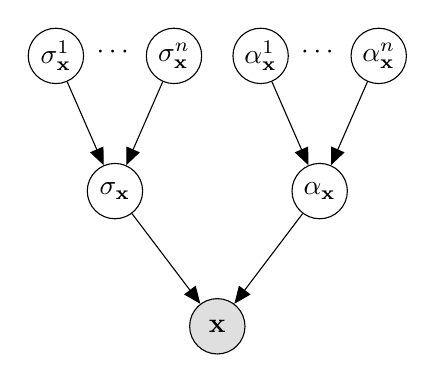
\begin{tikzpicture}
	% Define nodes
	\node[obs]                               (x) {$\mathbf{x}$};
	\node[latent, above=of x, xshift=-1.3cm] (z1) {$\sigma_{\mathbf{x}}$};
	\node[latent, above=of x, xshift=1.3cm]   (zn) {$\alpha_{\mathbf{x}}$};
	\node[latent, above=of zn, xshift=-0.75cm]   (sn) {$\alpha^1_{\mathbf{x}}$};
	\node[latent, above=of zn, xshift=0.75cm]   (an) {$\alpha^n_{\mathbf{x}}$};
	\node[latent, above=of z1, xshift=-0.75cm]   (s1) {$\sigma^1_{\mathbf{x}}$};
	\node[latent, above=of z1, xshift=0.75cm]   (a1) {$\sigma^n_{\mathbf{x}}$};
	% \node[latent, above=of x]   (zi) {$\mathbf{p_i}$};
	\node[auto=false, above=of z1, yshift=0.2cm] (dots) {$\cdots$}  ;
	\node[auto=false, above=of zn, yshift=0.2cm] (dots) {$\cdots$}  ;
	% \node[auto=false, above=of x, yshift=0.2cm, xshift=-0.6cm] (dots1) {$\cdots$}  ;
	% Connect the nodes
	\edge {z1,zn} {x} ; %
	\edge {a1,s1} {z1} ; %
	\edge {an,sn} {zn} ; %
	% Plates
	% \plate {yx} {(x)(y)} {$N$} ;
	% \plate {} {(w)(y)(yx.north west)(yx.south west)} {$M$} ;
\end{tikzpicture}


			\caption{Modelling an image of an object as a collection of parts, each with its own shape and appearance}
			\label{fig:s1}
		\end{subfigure}
		\begin{subfigure}{0.49\linewidth}
			\centering
			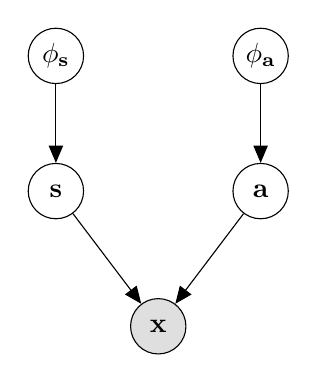
\begin{tikzpicture}
	% Define nodes
	\node[obs]                               (x) {$\mathbf{x}$};
	\node[latent, above=of x, xshift=-1.3cm] (s) {$\mathbf{s}$};
	\node[latent, above=of x, xshift=1.3cm]   (a) {$\mathbf{a}$};
	\node[latent, above=of s] (ts) {$\phi_\mathbf{s}$};
	\node[latent, above=of a] (ta) {$\phi_\mathbf{a}$};
	\edge {s,a} {x} ; %
	\edge {ts} {s} ; %
	\edge {ta} {a} ; %
	% Plates
	% \plate {yx} {(x)(y)} {$N$} ;
	% \plate {} {(w)(y)(yx.north west)(yx.south west)} {$M$} ;
\end{tikzpicture}



			\caption{Implementing the do-operation with a transformation of factors}
			\label{fig:s2}
		\end{subfigure}
		\caption{}
		\label{fig:fig}
	\end{figure}

	To capture an object in an abstract representation, we follow two key ideas: \emph{(i)} disassembling the object into its constituent parts and \emph{(ii)} disentangling spatial geometry (shape) from visual features (appearance). Hence, we model an object as a composition of parts, each part with a part appearance and a part shape, see Fig. \ref{fig:representation}. The part shape should correspond to the area in the image where the part is located, whereas the part appearance is a feature descriptor for that area. The overall object representation is then the collection of part shapes and part appearances. \\
	% \begin{equation}
	%(a, s) = \cup_i (f_i, p_i)
	%\end{equation}
	%\label{eq:representation}
	% enforcing locality of parts is important
	% what do our representations entangle still?:
	% shape: position, shape, size
	% appearance: illumination, color, texture, material
	\todo{local features theme}
	The disentanglement of shape and appearance can be enforced by demanding that shape is invariant under the transformation of appearance and vice versa. This is realized in a two-stream auto-encoding formulation. Here, an image is reconstructed from a combination of shape and appearance, with shape extracted from the appearance-transformed image and appearance from a shape-transformed image. Additionally, the part shape is tied to the location of the part in the image: an equivariance loss encourages that the part shape moves in unison with the part in the image. We implement these objectives into a loss framework, which is explained in sec. \ref{sec:framework}. \\
	To assert a decomposition into independent local parts, we ensure their local modelling and treatment throughout the whole pipeline. This is highlighted when describing the architecture in sec. \ref{sec:architecture}.

\section{Framework}\label{sec:framework}
	% CROSSING TASK FRAMEWORK
	\begin{figure}[t]
		\centering
		\includegraphics[trim={0cm 0cm 0cm 0cm},clip, width=1.\linewidth]{fig/architecture_final}
		\caption{Encoder $E$ encodes shape and appearance for two images $\pi(X)$ and $\phi(X)$, after recombination $R$ of $(f_{\pi(X)}, p_{\phi(X)})$ into latent image $Z$, the decoder $D$ reconstructs the image $X$.}
		\label{fig:framework}
	\end{figure}
	%Definitions
	We want to represent an object in an image $X$. Let us denote the part shape with $p_X$ and the part appearance with $f_X$. For an object with $n$ parts, the overall shape is constituted by the collection of its part shapes $p_X =  (p^1_X, ...,  p^n_X)$, the same goes for the appearance $f_X =  (f^1_X, ...,  f^n_X)$. We model the part appearances as feature vectors, the part shapes are chosen to be scalar fields like the image itself. Thereby one can establish a direct correspondence of locations in the image to locations in the shape representation.\todo{say the following or not?}\\
	%In contrast to other works, where object pose is often modeled by single points as landmarks, a representation based on a scalar field is much richer: whereas a landmarks inform about the exact position, the field-like representation also describes the size and shape of the object parts (see Fig.\ref{fig:representation}).
	% Transformations -> Crossing framework
	How do we disentangle the shape and appearance components in the representation? In general, a variation in shape will not affect appearance and vice versa. Thus, if we deliberately change shape without changing appearance, we can enforce the invariance of the appearance representation under such a change.
	We refer to these changes as shape transformations $\pi$, which, if applied to an image $X$, directly act on the underlying pixel space $\Lambda$.
	Along the same lines we can define appearance transformations $\phi$, which act on the image itself.
	The shape should be invariant under change of appearance, conversely, the appearance should be invariant under change of shape.
	In addition, the shape should transform in the same manner as the image.
	That means the shape representation is assumed to be equivariant under shape transformations.
	In summary:
	\begin{align}
		f_{\pi(X)}  &= f_{X} \tag{invariance of appearance}\\
		p_{\phi(X)} &= p_X  \tag{invariance of shape}\\
		p_{\pi(X)} &= \pi(p_X) \tag{equivariance of shape}
	\label{eq:invar}
	\end{align} % quad \forall i \leq n
	Our method builds on the auto-encoding paradigm, with part shapes and part appearances assuming the role of the latent code.
	To incorporate these constraints into the loss of an auto-encoder, we reconstruct an image $X$ not from the shape and appearance $(f_X, p_X)$ determined from the original image $X$, but from appropriately transformed images $(f_{\pi(X)}, p_{\phi(X)})$.
	If the invariance constraints, as formulated above, are fullfilled, these transformations do not change the latent code.
	Thus, the loss implicitly enforces invariance.
	To obtain shape and appearance, we encode both $\phi(X)$ and $\pi(X)$ with an encoder $\mathrm{E}$.
	And, after a recombination $\mathrm{R}$ (for details see sec. \ref{sec:architecture}) to a latent image $Z$, a decoder $\mathrm{D}$ reconstructs the image.
	This configuration is depicted in Fig. \ref{fig:framework}, the reconstruction loss $\mathcal{L}_{\textrm{rec}}$ is as follows:
	%\begin{align}
	%\mathcal{L}_{\textrm{rec}} &=  \lVert X -  \mathrm{D}[\mathrm{R}[\mathrm{E}(X)]]\rVert \\
	%&= \lVert  X  - \mathrm{D}[\mathrm{R}[ (f_X, p_X)]]\rVert \nonumber \\
	%&= \lVert  X  - \mathrm{D}[\mathrm{R}[ (f_{X_{\pi'}}, p_{X_{\phi'}}]]\rVert \nonumber
	%\end{align}
	%The to-be-reconstructed image $X_{\phi, \pi}$ has been subject to shape and appearance transformations $X \rightarrow \phi \circ \pi (X)$.
	%We instantiate this loss in a two-stream configuration, as shown in Fig. \ref{fig:framework}. %Encoder and decoder are the same for each stream, but image representations are crossed.
	%For simplicity we abbreviate $f = f_{\pi(X)}$, $f' = f_{\phi(X)}$ , $s = p_{\phi(X)}$ and $s' = p_{\pi (X)}$.
	%In accordance with the desired invariances, one can apply a transformation $\phi$ to the image, in order to selectively destroy appearance information in the shape representation and vice versa destroy shape information in the appearance representation with $\pi$.
	%The first stream encodes $\pi(X)$ to obtain $(a, s')$  and the second stream encodes $\phi(X)$ to obtain $(a', s)$.
	%Then appearance and shape representations are crossed.
	%After recombining $(a, s)$ to a feature volume $V$ (explained in detail in sec. \ref{sec:architecture}), the decoder reconstructs $X$.
	\begin{equation}
	\mathcal{L}_{\textrm{rec}}= \lVert  X  - \mathrm{D}[\mathrm{R}(f_{\pi(X)}, p_{\phi(X)})]\rVert
	\end{equation}
	\label{eq:loss_rec}
	%From an information perspective, we apply an appearance transformation to the image, to selectively destroy appearance information in the shape representation and vice versa destroy shape information in the appearance representation with a shape transformation.
	Let us examine what this formulation means on the level of a single part: the part appearance $f^i_X$ is extracted at locations in the spatially transformed image $p^i_{\pi(X)}$, but then used for reconstruction at the location in the original image $p^i_{X}$. For example in Fig.  \ref{fig:framework} the appearance of the arm will be extracted in a raised position, but then these features are used for reconstructing an arm in a lowered position. For this to succeed, firstly, the appearance features need to be sufficiently abstract. Secondly, part locations of the two images have to refer to the same part and track the location of it consistently. This part assignment consistency is an implicit way to improve equivariance under the shape transformations.\\
	%The shape also need to be invariant under appearance transformations, so part assignment needs to be consistent .
	%For video data the crossing task can be run on images pairs that show the same object in a different articulation (i.e. different frames of the video), enforcing equivariance of $s$ with respect to natural shape transformations. \\
	For a known shape transformation the equivariance of shape can also be encouraged explicitly with a loss. This has been used before in the context of unsupervised landmark learning by \cite{thewlis17, Zhang18} as a point-wise loss on a part probability map, encouraging the exact location of a part to transform accordingly. In our case, the part shapes shall not encode probability, but instead the spatial extend of a part. In approximation, we want the first two moments ($\mu, \Sigma$) to transform correctly. Thereby the extend and orientation of the parts is penalized in addition to the mere position.
	\begin{equation}
	\mathcal{L}_{\textrm{equiv}}^i = \mathcal{L}_{\mu}^i+ \mathcal{L}_{\Sigma}^i
	\label{covariance}
	\end{equation}
	The overall loss objective is the sum of the reconstruction loss and the equivariance loss for all $n$ parts:
	\begin{equation}
	\mathcal{L} = \sum_{i=1}^n \mathcal{L}_{\text{equiv}}^i + \mathcal{L}_{\textrm{rec}}
	\end{equation}


\section{Architecture}\label{sec:architecture}
	The auto-encoding pipeline consists of three stages, namely: \textbf{encoding} both shape and appearance for each part,  \textbf{recombining} this information meaningfully into a latent image and \textbf{decoding} this latent image to reconstruct the image. The whole process is sketched in Fig. \ref{fig:framework}, the operations in more detail are visualized in Fig. \ref{fig:x1}, \ref{fig:x2}, \ref{fig:x3},  \ref{fig:x4}. Throughout the procedure we maintain the local correspondence between the representation and the image: We ensure a local appearance extraction in the encoding, a local synthesis in the recombining and a local usage of the latent image in the decoding. These architectural restrictions enable a disentangled part representation with the interpretation of a part as a localized entity. \\

	\subsection{Analysis}
		${(f, p | X)}$\footnote{ For a slim notation, we leave out the explicit reference to the generic input image $X$ in this section: $f, p, f^i, p^i$ refer to $f_X, p_X, f^i_X, p^i_X$.} The encoding of shape and appearance given an image proceeds in two steps: \\
		\emph{(i.)} $(p|X)$: The part shapes are predicted given the image. To extract part shapes we use an hourglass\footnote{ We utilize hourglass neural network models in both steps, as these models are able to preserve pixel-wise locality, but integrate information from multiple scales \cite{hourglass}.}  neural network: The input is an image $X$, the output a stack of $n$ part shapes $s =  \{p^i| i=1, ...,  n\}$.\\ \emph{(ii.)} $(p|f,X)$: The part appearances $f =  \{f^i| i=1, ...,  n\}$ are predicted given the image and the part shapes. Again we use an hourglass network, albeit shallower. The input is the original image concatenated with the stack of part shapes. The output is a feature stack $F$. A part appearance is obtained by averaging the feature stack with the a part shape: $f^i = \sum_{x \in \Lambda} A(x) \frac{p^i(x)}{\sum_{x' \in \Lambda}p^i(x')} $. Each $f^i$ now describes the appearance of a part spatially localized by the part shape $p^i$. \\

	\subsection{Recombination of Factors}
		In the analysis-by-synthesis regime, once the object representation is successfully factorized, one can make assumptions on how the factors reunite to generate an image, following the knowledge and intuition about how objects give rise to images in the physical world.
		Firstly, we remerge shape and appearance into images of descriptors at the correct locations. For each part, appearance is multiplied with the corresponding shape, yielding $n$ part feature images: $z^i(x) = p^i(x) \cdot f^i$.
		Secondly, we reassemble the object from its parts: the part feature images $z^i$ are summarized by summing in a single image: $ Z(x) = \sum_i \frac{z^i(x)}{1 + \sum_j z^j(x)}$. The result is an image of part feature descriptors located according to their corresponding part shape, which we call latent image $Z$.\\


	\subsection{Synthesis}
		Finally, the latent image needs to be decoded to an image. This is done by a neural network decoder. The decoder architecture is modeled after the upsampling stream of a standard U-Net \cite{}. The latent image is scaled to different scales \todo{alter figure z1 etc} and inserted, after each layer, in addition to the part shapes \todo{why add shapes?}. As before, the crucial property of the parts that needs to be conserved is their local direct correspondence to the image. On the one hand, one needs to assure, that the receptive field of the neurons does not extend to the full image, in order to thwart a complex non-local interaction of part information. This is why we use only half of a U-Net instead of a complete U-Net or an hourglass architecture.
		On the other hand, it is essential to regularize the information already before passing it to the decoder. Keeping in mind that the part shape should be of rather simple geometry, we introduce a differentiable information bottlenecks, in order to prevent the shape from being scattered over the object. It is an approximation of the part shape as $\hat p^i(x) = \frac{1}{1 + (x -\mu)^T \Sigma^{-1} (x - \mu)}$, where $\mu$ and $\Sigma$ are the mean and the covariance matrix of the part shape $p^i$. This allows to pass second-order information such as size and orientation of the part to the decoder. Note that this operation are fully differentiable.


	\section{Implementation Details}\label{implementationdetails}
		The image resolution is $128 \times 128$, but the resolution of corresponding part shapes is $ 64 \times 64$. \\
		For the reconstruction  loss $\mathcal{L}_\text{rec}$ we use the $L_1$ or $L_2$ distance. To prevent parts from trying to explain the whole image, instead of focusing on the object, we also restrict the reconstruction loss to an area around the part shape: a sum of Gaussian approximations around the means of the part shapes is folded with the loss.\\
		In the decoder, the latent image Z is not only rescaled, but also filled with parts incrementally. At the lowest scale only some parts are inserted, with each scale parts are added until at the highest scale all parts are used. This makes the part decoding a hierarchical process. The underlying assumption is the parts exist at multiple scales.
		For landmark learning, we approximate the part shapes in the decoder in the bottleneck also with $\hat p^i(x) = \frac{1}{1 + (x -\mu)^T \Sigma^{-1} (x - \mu)}$, but fix the covariance $\Sigma$ to the identity matrix. Hence, effectively only information about the mean of each part shape can reach the decoder. This mean information is used as a landmark, so encouraging an accurate estimation of the mean through reconstruction is wanted.\todo{this needs further explanation or is dangerous}\\
		To instantiate shape transformations $\pi$, one needs image pairs that show the same object in a different articulation or position: For static images an artificial thin-plate spline transform (TPS) can be applied, which generalizes rotation, scaling, translation. For video data adjacent frames exhibit natural shape transformations. The appearance transformation $\phi$ is encompassing a colour augmentation, contrast variations, and changes in brightness. In general, the more selective the transformation distinguishes shape and appearance, the more invariant the representation.

	% %&tex

\chapter{Object Shape Learning}
	% PENN SHAPES
	\begin{figure}[htp]
		\begin{subfigure}{1.\textwidth}
		\centering
		\includegraphics[trim={0cm 0cm 0cm 0cm},clip, width=1.\linewidth]{fig/shape/shape8white}\caption{}
		\label{fig:shape_penn}
		\end{subfigure}
		\begin{subfigure}{1.\textwidth}
		\centering
		\includegraphics[trim={0cm 0cm 0cm 0cm},clip, width=1.\linewidth]{fig//shape/shape_yoga8}\caption{}
		\label{fig:shape_tennis}
		\end{subfigure}
		\caption{Learned shape representation on Penn Action. For visualization, 13 of 16 part activation maps are plotted in one image. (a) Different instances, showing intra-class consistency and (b) video sequence, showing consistency and smoothness under motion, although each frame is processed individually.}
		\label{fig:shape}
	\end{figure}

	A visualization of the learned shape representation is shown in Fig.~\ref{fig:shape}. \todo{ours region-based, landmarks only for evaluation}
	To quantitatively evaluate the shape estimation, we measure how well groundtruth landmarks (only during testing) are predicted from it.
	We obtain landmarks from our part-region based shape representation by designating the mean of a part shape $\mu[\sigma^i(\mathbf{x})]$ as the landmark position. To quantify the quality of these landmark estimates, we linearly regress them to human-annotated groundtruth landmarks and measure the test error.
	% The part shape means $\mu[\sigma^i(x)]$ serve as our landmark estimates and we measure the error when linearly regressing the human-annotated groundtruth landmarks from these estimates.
	For this, we follow the protocol of Thewlis \etal \cite{thewlis17}, fixing the network weights after training the model, extracting unsupervised landmarks and training a single linear layer without bias.
	The performance is quantified on a test set by the mean error and the percentage of correct landmarks (PCK).
	We extensively evaluate our model on a diverse set of datasets, each with specific challenges.
	On all datasets we outperform the state-of-the-art by a significant margin.\\

	In the following, we proceed through our shape learning results: we present the quantitative and qualitative \textit{results} by category (sec. \ref{sec:results}). On the way we introduce the datasets for each category. In the next section we highlight and discuss the \textit{challenges}, which the datasets present (sec. \ref{sec:challenges}) and subsequently argue for the importance of the \textit{transformations} as a means to overcome those challenges (sec. \ref{sec:transformations}).

\section{Diverse Object Categories}\label{sec:results}
	On the object classes of human faces, cat faces, and birds and human and animal bodies our model predicts landmarks consistently across different instances.

	\subsection{Human and Cat Faces}
		Due to different breeds and species the Cat Head, CUB-200-2011 exhibit large variations between instances. Especially on these challenging datasets we outperform competing methods by a large margin.
		Tab.~\ref{tab:faces} compares against the state-of-the-art.
		% RESULTS FACES
		\begin{table}[t]
			\caption{Error of unsupervised methods for landmark prediction on the Cat Head, MAFL (subset of CelebA) testing sets. The error is in \% of inter-ocular distance.}
			\label{tab:faces}
			\centering
			\begin{tabular}{l|ccc}
			\hline
			Dataset & Cat Head &  & MAFL \\
			  \# Landmarks &10 & 20  & 10  \\
			  \hline
			 Thewlis \cite{thewlis17}
			 & 26.76 & 26.94 & 6.32    \\
			 Jakab \cite{jakab18}
			 & - & - & 4.69  \\
			 Zhang \cite{zhang18}
			 & 15.35 & 14.84 & 3.46  \\
			  Ours & \textbf{9.88}  & \textbf{9.30} & \textbf{3.24}  \\ \hline  % image length is 600: 32.15 , 23.51
			\end{tabular}
		\end{table}

		% FACES
		\begin{figure}[htp]
			\centering
			\begin{subfigure}{1.\textwidth}
			\includegraphics[trim={0cm 0cm 0cm 0cm},clip, width=1.\linewidth]{fig/shape/0celeba}\caption{}
			\end{subfigure}
			\begin{subfigure}{1.\textwidth}
			\includegraphics[trim={0cm 0cm 0cm 0cm},clip, width=1.\linewidth]{fig/shape/0cats}\caption{}
			\end{subfigure}
			\caption{{Unsupervised discovery of landmarks the object classes of (a) human (CelebA dataset) and (b) cat faces (Cat Head dataset).}}
			\label{fig:kp_faces}
		\end{figure}

		\paragraph{CelebA} \cite{liu15facewild} contains ca. 200k celebrity faces of 10k identities.
		We resize all images to $128\times 128$ and exclude the training and test set of the MAFL subset, following \cite{thewlis17}.
		As  \cite{thewlis17, zhang18}, we train the regression (to 5 ground truth landmarks) on the MAFL training set (19k images) and test on the MAFL test set (1k images).

		\paragraph{Cat Head} \cite{zhang08cathead}  has nearly 9k images of cat heads.
		We use the train-test split of \cite{zhang18} for training (7,747 images) and testing (1,257 images).
		We regress 5 of the 7 (same as \cite{zhang18}) annotated landmarks.
		The images are cropped by bounding boxes constructed around the mean of the ground truth landmark coordinates and resized to $128\times128$.

	\subsection{Human Bodies}
		% BODIES
		\begin{figure}[htp]
			\centering
			\begin{subfigure}{1.\textwidth}
			\includegraphics[trim={0cm 0cm 0cm 0cm},clip, width=1.\linewidth]{fig/shape/0human}\caption{}
			\end{subfigure}
			\begin{subfigure}{1.\textwidth}
			\includegraphics[trim={0cm 0cm 0cm 0cm},clip, width=1.\linewidth]{fig/shape/0penn}\caption{}
			\end{subfigure}
			\caption{{Unsupervised discovery of landmarks the object classes of human bodies (a) in constrained (Human3.6M dataset) and (b) unconstrained environments (Penn Action dataset).}}
			\label{fig:kp_bodies}
		\end{figure}


		% BBC POSE Results
		\begin{table}[t]
			\caption{{
			Performance of landmark prediction on BBC Pose test set. As upper bound, we also report the performance of supervised methods.
			%Comparing against supervised and unsupervised methods for annotated landmark prediction on the BBC Pose testing set.
			The metric is \% of points within 6 pixels of groundtruth location. %Note that Jakab et al. are using a 50-landmarks, while we only use a 30 landmarks as input for the regression.
			}}
			\label{tab:bbcpose}
			\centering
			\begin{tabular}{ll|cr}
			\hline
			BBC Pose &   &    { Accuracy}  \\
			 \hline
			supervised & Charles \cite{charles13bbcpose} &
			   79.9\%  \\ % 79.90
			 & Pfister \cite{pfister15flowingconv}  &
			  88.0\%  \\ \hline % 88.01
			unsupervised &Jakab \cite{jakab18} &
			 68.4\%  \\  % 68.44
			  &Ours &  \textbf{74.5}\% \\
			% test pck = 0.7484605918670523
			% test pck_per_kp = [0.9633621  0.6627155  0.76508623 0.54956895 0.6928879  0.76616377   0.83943963]
			\hline
			\end{tabular}
		\end{table}

		% HUMAN3.6M Results
		\begin{table}[t]
			\caption{{Comparing against supervised, semi-supervised and unsupervised methods for landmark prediction on the Human3.6M test set. The
			error is in \% of the edge length of the image. All methods predict 16 landmarks.
			}}
			\label{tab:human}
			\centering
			\begin{tabular}{ll|cr}
			\hline
			 Human3.6M   & &  { Error w.r.t. image size}  \\
			 \hline
			 supervised & Newell \cite{newell16hourglass}
			  &2.16  \\  \hline
			 semi-supervised & Zhang \cite{zhang18}
			  & 4.14  \\ \hline
			 unsupervised & Thewlis \cite{thewlis17}
			 & 7.51  \\
			  & Zhang \cite{zhang18}
				& 4.91 \\
			  & Ours& \textbf{2.79} \\
			\hline
			\end{tabular}
		\end{table}


		\paragraph{BBC Pose} \cite{charles13bbcpose} contains videos of sign-language signers with varied appearance in front of a changing background. Like \cite{jakab18} we loosely crop around the signers.
		The test set includes 1000 frames and the test set signers did not appear in the train set.
		For evaluation, as \cite{jakab18}, we utilized the provided evaluation script, which measures the PCK around $d=6$ pixels in the original image resolution.


		\paragraph{Human3.6M} \cite{ionescu14human36m} features human activity videos.
		We adopt the training and evaluation procedure of \cite{zhang18}.
		For proper comparison to \cite{zhang18} we also removed the background using the off-the-shelf unsupervised background subtraction method provided in the dataset.


		\paragraph{Penn Action} \cite{zhang13penn} contains 2326 video sequences of 15 different sports categories.
		For this experiment we use 6 categories (tennis serve, tennis forehand, baseball pitch, baseball swing, jumping jacks, golf swing).
		We roughly cropped the images around the person, using the provided bounding boxes, then resized to $128\times128$.

	\subsection{Animal Bodies}
		% RESULTS BIRDS
		\begin{table}[t]
			\caption{Error of unsupervised methods for landmark prediction on the CUB-200-2011 testing set.
			The error is in \% of edge length of the image.}
			\label{tab:static}
			\centering
			\begin{tabular}{l|cccc}
				\hline
				Dataset &  & CUB-200-2011\\
				\# Landmarks & 10  \\
				\hline
				Zhang \cite{zhang18} & 5.36 \\
				Ours  & \textbf{3.91}  \\ \hline
			\end{tabular}
		\end{table}


		% DOGS, BIRDS
		\begin{figure}[htp]
			\centering
			\begin{subfigure}{1.\textwidth}
			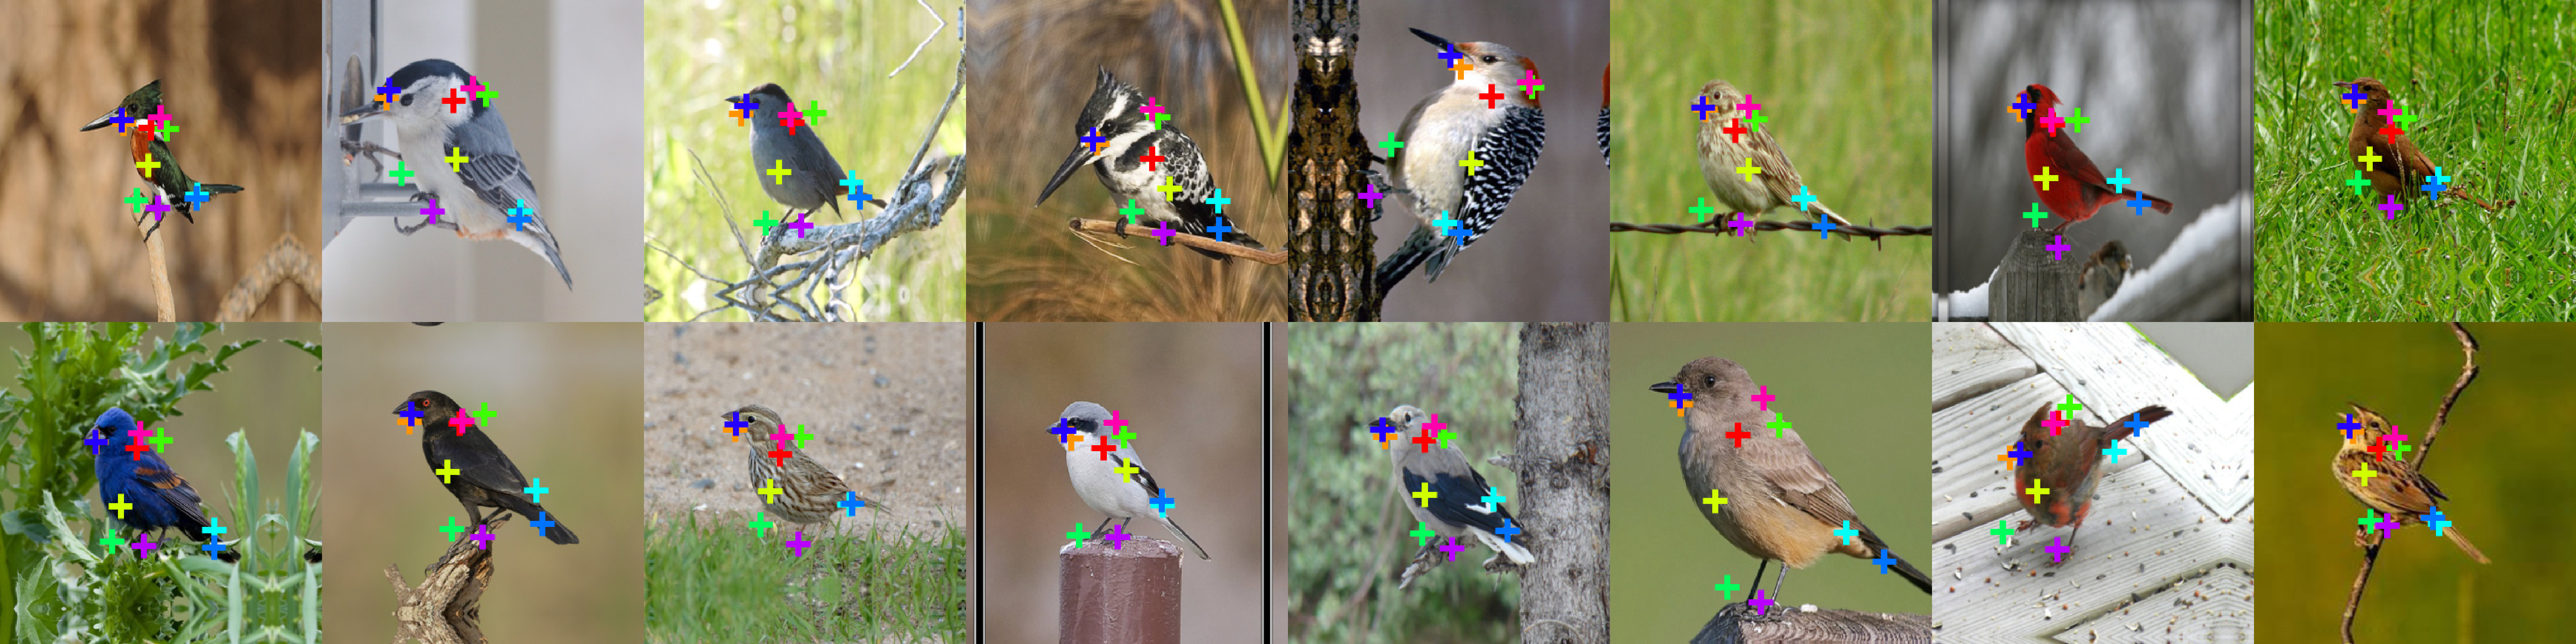
\includegraphics[trim={0cm 0cm 0cm 0cm},clip, width=1.\linewidth]{fig/shape/0birds}\caption{}
			\end{subfigure}
			\begin{subfigure}{1.\textwidth}
			\includegraphics[trim={0cm 0cm 0cm 0cm},clip, width=1.\linewidth]{fig/shape/0dogs}\caption{}
			\end{subfigure}
			\caption{{Unsupervised discovery of landmarks the object classes of animal bodies (a) birds (CUB-200-2011 dataset) and (b) dogs (Dogs Run dataset).}}
			\label{fig:kp_animals}
		\end{figure}


		\paragraph{CUB-200-2011} \cite{wah11birds} comprises ca. 12k images of birds in the wild from 200 bird species.
		We excluded bird species of seabirds, roughly cropped using the provided landmarks as bounding box information and resized to $128\times128$.
		We aligned the parity with the information about the visibility of the eye landmark.
		For comparing with \cite{zhang18} we used their published code.


		\paragraph{Dogs Run} is made from dog videos from YouTube totaling in 1250 images under similar conditions as in Penn Action. The dogs are running in one direction in front of varying backgrounds. The 17 different dog breeds exhibit widely varying appearances.

	\section{Challenges}\label{sec:challenges}
		An overview over the challenges implied by each dataset is given in Tab.~\ref{tab:challenges}.

		We demonstrate (Fig. \ref{fig:kp_mania}), that our model not only exhibits strong landmark consistency under articulation, but also covers the full human body meaningfully.
		Even fine-grained parts such as the arms are tracked across heavy body articulations, which are present in the Human3.6M or Penn Action datasets.
		Also with further complications such as viewpoint variations, blurred limbs and partial self-occlusions we are able to detect landmarks on Penn Action of similar quality and coverage as in the more constrained Human3.6M dataset.
		Additionally, complex background clutter, as in BBC Pose and Penn Action, does not hinder finding the object.
		The Dogs Run dataset displays that even completely different dog breeds can be related via semantic parts.
		% Here, the universality of the approach (capturing non-human poses) is underlined once more.
		% This is to be expected, as no prior assumptions about the object-class are introduced in the model.
		% Furthermore, the limited amount of data in Dogs Run is no problem for finding meaningful correspondences, due to the unsupervised nature of the model and the transformations acting as a form of data augmentation. \\
		% Quantitative evaluation is shown on Human3.6M against \cite{Zhang:2018vz, Thewlis:2017wi} (Tab. \ref{tab:human}), on BBC Pose against \cite{Jakab:2018wc} (Tab. \ref{tab:bbcpose}). Qualitatively, we show additional landmark discovery results on Penn Action and on the Dogs Run video dataset.\\
		The quantitative results are shown in Tab. \ref{tab:bbcpose} and Tab. \ref{tab:human}: other unsupervised and semi-supervised methods are outperformed by a large margin on both datasets.
		%On Human3.6M, judging by the performance gap, it is questionable whether the other unsupervised method (\cite{Thewlis:2017wi}) learned to deal with articulation at all.
		% On Human3.6M, Zhang et al. \cite{Zhang:2018vz} additionally used optical flow to stabilize their training, which we classified as semi-supervised. %which provides a significant information advantage compared to our approach.
		On Human3.6M, our approach is able to achieve a large performance gain even over results obtained with optical flow supervision. %The  relative position and errors of our landmarks compared to the manually annotated landmarks are shown in Fig. \ref{fig:regress}.
		On BBC Pose, we outperform \cite{Jakab:2018wc} by $6.1\%$, reducing the performance gap to supervised methods significantly.

		%DATASET CHALLENGES
		\begin{table}
			\centering
			\caption{Difficulties of datasets: articulation, intra-class variance, background clutter and viewpoint variation}
			\label{tab:challenges}
			\begin{tabular}{l|rrrr}
				\hline
				Dataset &  Articul.& Var. &  Backgr.& Viewp.  \\ \hline
				CelebA &   &  &  &    \\
				Cat Head & &  \checkmark&  &   \\
				CUB-200-2011 & & \checkmark& \checkmark&   \\
				Human3.6M &\checkmark& &  & \checkmark  \\
				BBC Pose &  \checkmark&  & \checkmark&  \\
				Dogs Run & \checkmark& \checkmark& \checkmark&   \\
				Penn Action & \checkmark& \checkmark& \checkmark& \checkmark  \\
				\hline
			\end{tabular}
		\end{table}
		\subsection{Composite Objects/Scenes}
			What is an object? What is a scene?
			compositional nature of reality
			Bird on twig object? Bird can also fly, but neural networks learn by correlation in data (-> ref to these failure modes)
			Dancing pair as object.
		\subsection{Object/Background Separation}
			Complexly cluttered background - as long as no correlations to the object exist - is actually favorable for the method. Correlations of object with background will belong to object.
		\subsection{Object Articulation}
			Object articulation makes consistent landmark discovery challenging.
			Fig. \ref{fig:kp_mania} shows that our model exhibits strong landmark consistency under articulation and covers the full human body meaningfully.
			Even fine-grained parts such as the arms are tracked across heavy body articulations, which are frequent in the Human3.6M and Penn Action datasets.
			Despite further complications such as viewpoint variations or blurred limbs our model can detect landmarks on Penn Action of similar quality as in the more constrained Human3.6M dataset.
			Additionally, complex background clutter as in BBC Pose and Penn Action, does not hinder finding the object.
			Experiments on the Dogs Run dataset underlines that even completely dissimilar dog breeds can be related via semantic parts.
			Tab. \ref{tab:bbcpose} and Tab. \ref{tab:human} summarize the quantitative evaluations: we outperform other unsupervised and semi-supervised methods by a large margin on both datasets.
			On Human3.6M, our approach achieves a large performance gain even compared to methods that utilize optical flow supervision.
			On BBC Pose, we outperform \cite{jakab18} by $6.1\%$, reducing the performance gap to supervised methods significantly.
		\subsection{Intra-Class Variation}
		on cat head, human mislabelling is the most common failure mode

\section{Transformations}\label{sec:transformations}
	\note{in this section: effect of transformations on learning, disentangling}
	\note{effectively connecting samples from the dataset, spreading the}
	\note{schedule transformations with exponential}

	\subsubsection{Parity}
	birds parity
	salsa parity

	\subsubsection{Rotation, Scaling, Translation}
		on Cats -> black cats different set of KP than rest -> connect these samples via transformation to reach intra-class consistency

	\subsubsection{Mimicking Appearance}

	% COLOR
	\begin{figure}[htp]
		\centering
		\includegraphics[trim={0cm 0cm 0cm 0cm},clip, width=.8\linewidth]{fig/shape/coloraugm}
		\caption{Examples for shape and appearance transformation on CUB-200-2011.}
		\label{fig:compare}
	\end{figure}


	Color, Contrast, Hue
	\subsection{Natural Changes in Video Data}
	Video data: Penn, Own
	% COMPARE ZHANG
	\begin{figure}[htp]
		\centering
		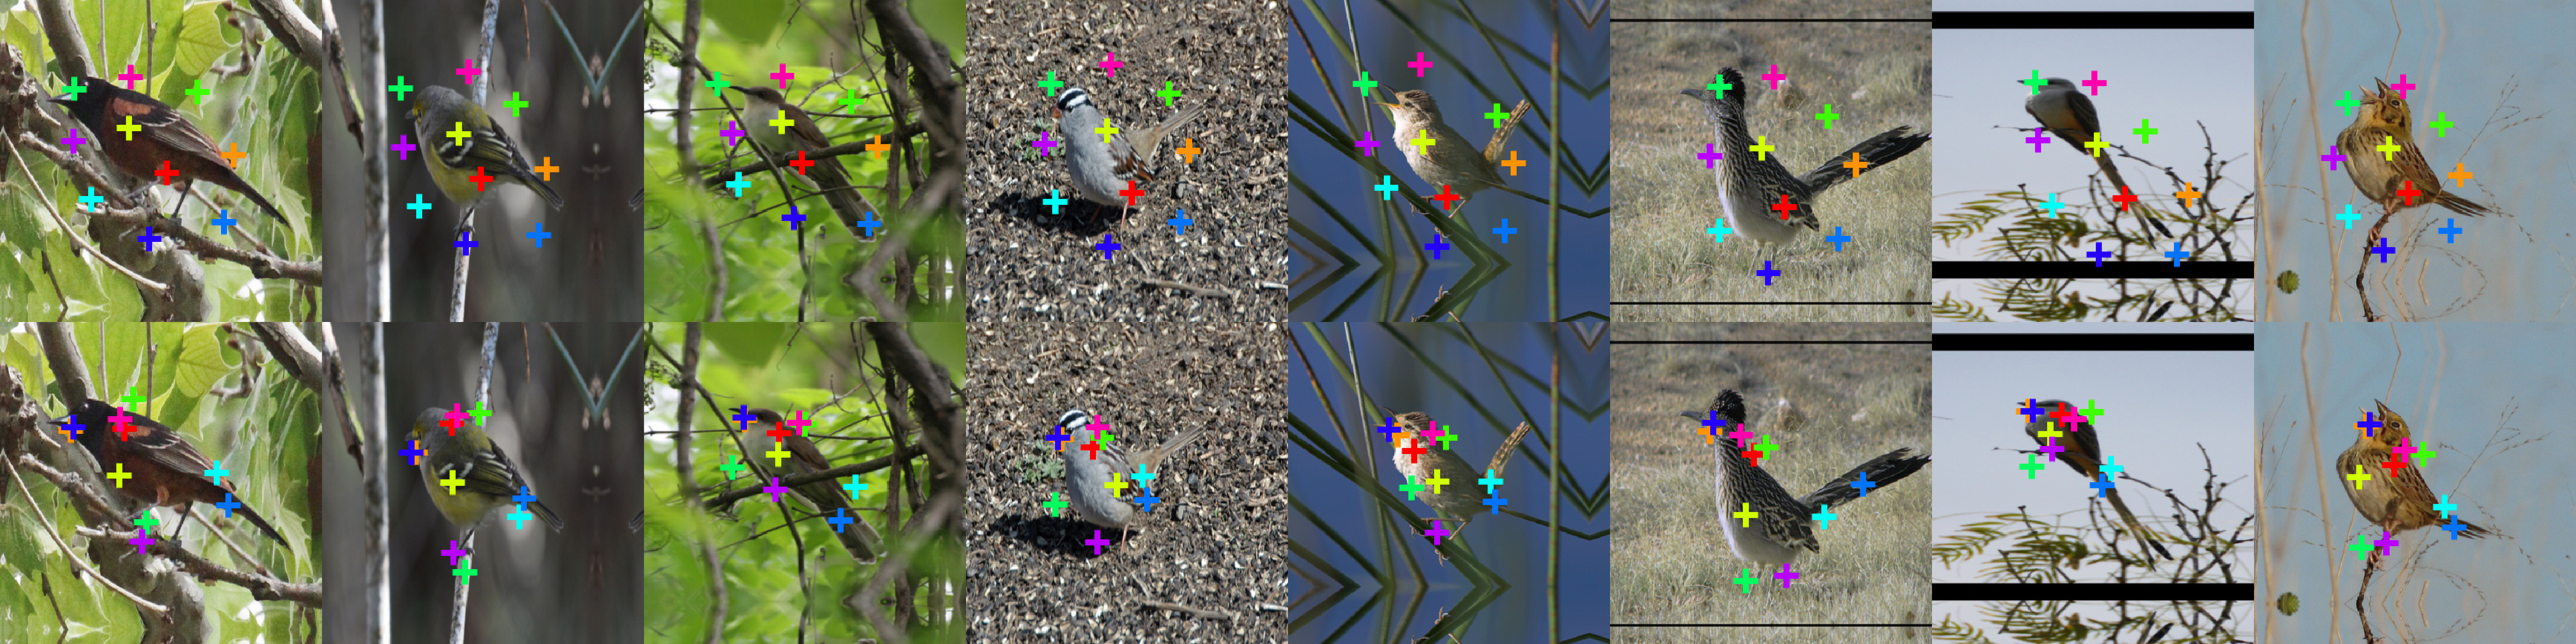
\includegraphics[trim={0cm 0cm 0cm 0cm},clip, width=1.\linewidth]{fig/shape/comp}
		\caption{Comparing discovered keypoints against \cite{zhang18} on CUB-200-2011. We improve on object coverage and landmark consistency. Note our flexible part placement compared to a rather rigid placement of \cite{zhang18} due to their part separation bias.}
		\label{fig:compare}
	\end{figure}

	Fig. \ref{fig:compare} provides a direct visual comparison to \cite{zhang18} on CUB-200-2011. It becomes evident that our predicted landmarks track the object much more closely. In contrast, \cite{zhang18} have learned a slightly deformable, but still rather rigid grid.
	This is due to their separation constraint, which forces landmarks to be mutually distant. We do not need such a problematic bias in our approach, since the localized, part-based representation and reconstruction guides the shape learning and captures the object and its articulations more closely.



	\subsection{Ablating Contributions}\label{sec:ablation}
	% ABLATION STUDY
	\begin{table}
		\centering
		\begin{tabular}{l|cr}
			\hline
			Dataset & Cat Head    \\
			\# Landmarks &  20 \\ \hline
			full model &  9.30 \\ \hline
			w/o $\mathcal{L}_{\textrm{eq}}$   & 11.32 \\
			w/o $\mathcal{L}_{\textrm{rec}}$   & 35.0 \\
			w/o appearance transform & 12.46 \\
			w/o shape transform & 14.72 \\ \hline
		\end{tabular}
		\caption{{Ablation studies on Cat Head dataset. We ablate the reconstruction loss $\mathcal{L}_{\textrm{rec}}$, equivariance loss $\mathcal{L}_{\textrm{eq}}$, the color augmentation and the crossing task}}
		\label{tab:ablation}
	\end{table}

	% what is the color augmentation: explain before
	\todo{what is the crossing task}
	We ablate the main components of our proposed framework: reconstruction loss $\mathcal{L}_{\textrm{rec}}$, the equivariance loss $\mathcal{L}_{\textrm{eq}}$, the appearance augmentation and the crossing task for disentangling shape and appearance. For the ablation study we use the Cat Head dataset, following the already introduced train-test setup on the task of landmark ground truth regression. Tab. \ref{tab:ablation} illustrates the ablation results.\\
	Leaving out the reconstruction task naturally leads to the largest drop in performance since only training on equivariance leads to collapsed landmark solutions as discussed in \cite{zhang18}.
	Training our model without color augmentations or appearance crossing between image pairs (i.e. the crossing task) weakens, respectively neglects the disentanglement of appearance and shape and hence the performance of our model significantly. % here specifically tackling intra-class variance
	Note that without the crossing task our models performs on par with Zhang \etal \cite{zhang18}, indicating, that this novel task could be explaining overall performance gain \wrt \cite{zhang18}. %This performance drop would be larger on datasets with articulation.
	Leaving out the explicit equivariance leads to the smallest drop in performance. This is not surprising, as equivariance is implicitly also enforced in the crossing framework.
	% without local features (not done yet, should we?, could ablate local decoder, or part appearance)

	\subsection{Crucial role of Transformations}

	The proposed method enables to abstract away object appearance from shape.
	Despite the multifarious challenges in the diverse range of datasets, the method is able to learn a dedicated part representation for shape.
	We compare to other approaches and reach state-of-the-art performance on the task of regressing human-annotated landmarks from the part representation.
	The key difference to the most competitive approach \cite{zhang18} is the emphasis on disentanglement via a crossed reconstruction with shape and appearance transformations.
	Enforcing disentanglement via targeted transformations enhances the shape representation in two ways: \emph{(i)} it asserts that no appearance information is encoded in the shape representation and vice versa and \emph{(ii)} it requires visual features to be equivariant under a spatial transformation.
	With regards to the considerations earlier, the crucial role of the transformations are to be expected, as they enable to reach a \textit{disentanglement}.


	% %&tex
\chapter{Disentanglement of Shape and Appearance}\label{sec:disentangling}
	Disentangled representations of object shape and appearance allow to alter both properties individually to synthesize new images. The ability to flexibly control the generator allows, for instance, to change the pose of a person or their clothing. In contrast to previous work \cite{esser18, denton17disvideo, ma17poseguided, ma17disperson, debem18dgpose, jakab18},
	we achieve this ability without requiring supervision \textit{and} using a flexible part-based model instead of a holistic representation. This allows to explicitly control the parts of an object that are to be altered. We quantitatively compare against \emph{supervised} state-of-the-art disentangled synthesis of human figures. Also we qualitatively evaluate our model on unsupervised synthesis of still images, video-to-video translation, and local editing for appearance transfer.
	\todo{incorporate following to make more expressive}
	% In this section we provide evidence that the proposed object factorization into local parts with shape and appearance components is indeed achieved by our model.
	% As is common for supervised disentangling methods, to evaluate the disentanglement of internal factors, we use the generated images to access the internal representation.
	% The global disentanglement of shape and appearance is tested on the task of conditional image generation and video-to-video translation, while the local part-wise disentanglement is tested on the task of part appearance transfer. \\
	% \textbf{Conditional Image Generation}
	% In a disentangled representation of object shape and appearance it should be possible to generate from the same shape with different appearances and vice versa.
	% In our model we can choose the shape or appearance conditioning by providing images as input to the shape or the appearance stream.

\section{Disentangling Pose and Appearance}\label{sec:poseandappearance}
		% POSE APPEARANCE SWAP
		\begin{figure}[htp]
			\centering
			\includegraphics[trim={0cm 0cm 0cm 0cm},clip, width=.5\linewidth]{fig/factor/swappy}
			\caption{Transferring shape and appearance on Deep Fashion. Without annotation the model estimates shape, 2nd column. Target appearance is extracted from images in top row to synthesize images. Note that we trained without image pairs only using synthetic transformations.
			%for training we had no image pairs but only synthetic transformations.
			%without being explicitly trained for this task.
			All images are from the test set.}
			\label{fig:allswaps}
		\end{figure}

		On Deep Fashion \cite{liu16deepfashion, liu16deepfashionwild}, a benchmark dataset for supervised disentangling methods, the task is to separate person ID (appearance) from body pose (shape) and then synthesize new images for previously unseen persons from the test set in eight different poses. We randomly sample the target pose and appearance conditioning from the test set. Fig. \ref{fig:allswaps} shows qualitative results.
		\todo{incorporate note}
		\note{We compare the disentangling performance quantitatively against a supervised method, namely the variational U-Net \cite{Esser:2018ue}. We evaluate on the DeepFashion dataset, a standard benchmark dataset for supervised disentangling methods. In this dataset appearance is defined by a persons ID and shape by the pose of the person. For each ID in the test set, we condition the image generation on 8 different poses which are chosen randomly from the test set. Both VU-Net and our model are conditioned on the exactly the same pose-ID image pairs.
		We quantitatively compare against supervised state-of-the-art disentangling \cite{esser18} by evaluating \emph{i)} invariance of appearance against variation in shape by the re-identification error and \emph{ii)} invariance of shape against variation in appearance by the distance in pose between generated and pose target image.}

		\begin{tcolorbox}
			\textbf{Deep Fashion} \cite{liu16deepfashion, liu16deepfashionwild} consists of ca. 53k in-shop clothes images in high-resolution of $256 \times 256$. We selected the images which are showing a full body (all keypoints visible, measured with the pose estimator by \cite{cao17affinityfield}) as full visibilty of the object is an assumption to the model and used the provided train-test split. For comparison with Esser \etal \cite{esser18} we used their published code.
		\end{tcolorbox}

	\subsection{Person Re-Identification}

		Person re-identification (ReID) is a research field on its own (overview in \eg \cite{almazan18reidtowards, bedagkar14reidtrends}), the goal being to learn a similarity metric for a persons appearance, invariant to a persons posture and the image viewpoint.
		% zheng16reidcnn
		The key applications are automated person tracking and surveillance \cite{zheng16reidfuture}.
		For our purposes, we will treat a ReID algorithm as a metric for measuring the preservation of appearance as well as the invariance to shape on our generated images.
		For this, we fine-tune an ImageNet-pretrained \cite{russakovsky15imagenet} Inception-Net \cite{szegedy15inception} with a ReID algorithm \cite{xiao17reidjoint} via a triplet loss \cite{hermans17reidtriplet} to the Deep Fashion training set.
		On the generated images we report the standard metrics for ReID, mean average precision (mAP) and rank-1, -5, and -10 accuracy.
		\todo{explain these metrics}
		% These metrics express
		% In single-image ReID the task is to
		% many-image ReID
		% ReID means ranking. rank-1 is the ratio of correct finding by the first entry. rank-n ratio of correct samples that are within first n entries in ranking. mean average precision is the average over
		The first question we ask, is, if the appearance encoding is stable to variations in pose, hence invariant to pose (shape). Each ID from the test set is generated in 8 different poses. The task for the ReID algorithm is now to rank the similarity of these pose-changed yet same-appearance generations.
		Although our approach is unsupervised, it is competitive compared to the supervised VU-Net \cite{esser18} as shown in Tab. \ref{tab:reid}. The high chance of reidentifying a persons appearance in a different shape (rank-1 accuracy) shows that the appearance is invariant against variation in shape (pose) for both methods.
 		To visualize the closeness of the same-ID generations in the ReID-embedding the show a t-SNE plot in Fig.~\ref{fig:tsne}.

		\begin{table}[htp]
			\centering
			\caption{Mean average precision (mAP) and rank-n accuracy for person re-identification on synthesized images after performing shape/appearance swap. Input images from Deep Fashion test set. Note \cite{esser18} is supervised \wrt shape.}
			\label{tab:reid}
			\begin{tabular}{l|cccr}
				\hline
				& mAP & rank-1 & rank-5 & rank-10 \\ \hline
				VU-Net \cite{esser18} & 88.7\% & 87.5\% & {98.7}\% & {99.5}\% \\
				Ours & {90.3}\% & {89.4}\% &{98.2}\% & {99.2}\% \\ \hline
			\end{tabular}
		\end{table}

		% TSNE
		\begin{figure}[htp]
			\centering
			\begin{subfigure}{0.49\linewidth}
			\includegraphics[trim={0cm 0cm 0cm 0cm},clip, width=1.0\linewidth]{fig/factor/tsne_img}
			\end{subfigure}
			\begin{subfigure}{0.49\linewidth}
			\includegraphics[trim={0cm 0cm 0cm 0cm},clip, width=1.0\linewidth]{fig/factor/tsne_bubble}
			\end{subfigure}
			% \begin{subfigure}{0.49\linewidth}
				% % \begin{subfigure}{0.49\linewidth}
				% \includegraphics[trim={0cm 0cm 0cm 0cm},clip, width=1.0\linewidth]{fig/factor/tsne10}
				% \end{subfigure}\begin{subfigure}{0.49\linewidth}
				% \includegraphics[trim={0cm 0cm 0cm 0cm},clip, width=1.0\linewidth]{fig/factor/tsne15}
				% \end{subfigure}
				% \begin{subfigure}{0.49\linewidth}
				% \includegraphics[trim={0cm 0cm 0cm 0cm},clip, width=1.0\linewidth]{fig/factor/tsne20}
				% \end{subfigure}
				% \begin{subfigure}{0.49\linewidth}
				% \includegraphics[trim={0cm 0cm 0cm 0cm},clip, width=1.0\linewidth]{fig/factor/tsne100}
				% \end{subfigure}
			% \end{subfigure}
			\caption{Visualization of feature distribution for generated person IDs. (Right) t-SNE (perplexity 16) of 10 generated IDs, (left) color-coded t-SNE (perplexity 12) for 10, 15, 20 and 100 IDs. Each ID has 8 samples. The different IDs are clearly separable, despite variation in pose: Hence, generated appearance is invariant to pose.}
			\label{fig:tsne}
		\end{figure}

		The second question one could ask is, if appearance is preserved, \ie if the ReID algorithm is able to reidentify the groundtruth appearance image from the generation. Results for this are shown in Tab.~\ref{tab:reiddirect}. The result depends strongly on whether the algorithm had been fine-tuned to the DeepFashion image distribution or the DeepFashion and the synthesized image distribution. The stark difference can be explained by the difference in the feature distribution: high-frequency details (such as patterns and texture of clothing), are not synthesized correctly, as the model is trained by a reconstruction objective which will blurr these high frequencies. On the other hand, the adversarial objective will encourage \textit{some} high frequencies, but not necessarily the ones from the initial appearance conditioning. The ReID algorithm, if not additionally adjusted to this, will pay attention to those details and subsequently fail.
		unambiguous function between generations and groundtruth can be found.

		\begin{table}[htp]
			\centering
			\caption{Mean average precision (mAP) and rank-n accuracy for person re-identification from synthesized to ground truth appearance images after performing shape/appearance swap. When only fine-tuning the ReID algorithm on DeepFashion, results are much worse that when also adjusting to the synthesized images.}
			\label{tab:reiddirect}
			\begin{tabular}{l|cccr}
				\hline
				Fine-tune to: & mAP & rank-1 & rank-5 & rank-10 \\ \hline
				% VU-Net \cite{esser18} & 88.7\% & 87.5\% & {98.7}\% & {99.5}\% \\
				DeepFashion & {17.2}\% & {25.4}\% &{48.8}\% & {60.4}\% \\
				DeepFashion and Synthesized Images& {75.0}\% & {73.8}\% &{89.5}\% & {92.5}\% \\ \hline
			\end{tabular}
		\end{table}



		\subsection{Pose Estimation}
		% \begin{figure}[htp]
			% \centering
			% \begin{subfigure}{0.49\linewidth}
			% \includegraphics[trim={0cm 0cm 0cm 0cm},clip, width=1.0\linewidth]{fig/pck18}
			% \end{subfigure}
			% \begin{subfigure}{0.49\linewidth}
			% \includegraphics[trim={0cm 0cm 0cm 0cm},clip, width=0.7\linewidth]{fig/factor/pck25}
			% \end{subfigure}
			% \caption{PCK Curve for VU-Net \cite{esser18} and Ours for re-estimating pose with a 25 keypoint human pose detector.}
			% \label{fig:pckcurve}
		% \end{figure}

		\begin{table}[htp]
			\centering
			\caption{Percentage of Correct Keypoints (PCK) for pose estimation on shape/appearance swapped generations.\;$\alpha$ is pixel distance divided by image diagonal. Note that \cite{esser18} serves as upper bound, as it uses the groundtruth shape estimates.}
			%shape supervision.}
			\label{tab:pose}
			\begin{tabular}{l|cccr}
				\hline
				$\alpha$ & $2.5\%$ &  $5\%$ & $7.5\%$ & $10\%$ \\ \hline
				VU-Net \cite{esser18} & {95.2}\% & {98.4}\% & {98.9}\% & {99.1}\% \\
				Ours & 85.6\% & 94.2\% &96.5\% & 97.4\% \\ \hline
			\end{tabular}
		\end{table}


		To evaluate shape, we extract keypoints using a pose estimator \cite{cao17affinityfield}. Tab. \ref{tab:pose} reports the difference between generated and pose target in percentage of correct keypoints (PCK).
		% , Fig. \ref{fig:pckcurve} shows the comparison of PCK curves.
		As would be expected, VU-Net performs better, since it is trained with exactly the keypoints of \cite{cao17affinityfield}. Nevertheless, our approach achieves an impressive PCK without supervision underlining value of the embedding of object shape and the disentanglement of appearance and shape. Despite random variation in appearance the shape does not change, this can also be directly observed from the conditioned generations in Fig.~\ref{fig:allswaps}.



\section{Disentangling in a Temporal Sequence}\label{sec:videotovideo}

	\begin{figure}[htp]
		\centering
		\includegraphics[trim={0cm 0cm 0cm 0cm},clip, width=1.\linewidth]{fig/factor/bbc_arrange}
		\caption{Generation results for conditioning appearances (top row) on pose (bottom, rightmost) on BBCPose.
		% The target appearances are from the train set, while the target pose is from the test set.
		Note that even fine-grained details in shape, such as fingers and facial expression are accurately captured.}
		\label{fig:bbcthumb}
	\end{figure}



	Conditional image generation can also be extended to the task of {video-to-video translation}. The two conditioning images can be frames from different videos. One frame is acting as the appearance conditioning and the other as shape conditioning. By generating each frame conditioned on the shape and appearance from two videos, one effectively transfers the appearance of one video to the shape of the other on a frame-to-frame level.
	We evaluate this frame-to-frame video translation on the BBCPose dataset. The datasets videos of sign language present a delicate and complex articulation of arms and hands. We condition on appearance from videos in the training set and on shape from videos in the test set. A sample for generated frames is shown in Fig. \ref{fig:bbcthumb}, for the complete videos please refer to the supplementary.
	We want to point out two features of the model here: Firstly, despite no use of smoothing or interpolation between frames the generated sequence is smooth in the temporal domain. This is enabled by a temporally consistent part assignment which is stable across articulation.
	Secondly, the training on the natural spatial transforms in video data enables the model to encapsulate realistic transitions such as out-of-plane rotation and complex 3D articulation of \eg hands and even fingers (note the correct translation of the thumbs position in Fig. \ref{fig:bbcthumb}). \\
	% \begin{itemize}
		% \item video-translation on BBCPose (frame-to-frame shape-appearance swap)
			% \begin{itemize}
				% \item $\Rightarrow$ shows realistic 3D transitions can be encapsulated in model by explicitly training on them (video data)
				% \item NO additional smoothing for frame-to-frame translation
					% $\Rightarrow$ latent space is consistent and smooth across time
			% \end{itemize}
	% \end{itemize}

\section{Part-wise Disentanglement}\label{sec:partwise}
	The second type of disentanglement we approach is to factorize the object into local parts. Obviously, object parts are in general not disentangled factors in a sense that they have an independent probability distribution\todo{ref to equation independence in beginning}. Since the parts are geometrically connected, in their spatial layout they are conditioned on each other. For example, you cannot move your head arbitrarily far away from your shoulders. Still, there is a local freedom and modularity - especially in appearance features - that renders a local factorization efficient. As an illustration, the color of the shoes you wear need only be mildly correlated with your hair color.
	We show that the model disentangles these local modes of variation for a persons appearance (Sec.~\ref{sec:partappearance}) and shape (Sec.~\ref{sec:partshape}).

	\subsection{Part-wise Appearance Transfer}\label{sec:partappearance}
	% PART SWAPS
	\begin{figure}[htp]
		\begin{subfigure}{0.49\linewidth}
		\centering
		\includegraphics[trim={0cm 0cm 0cm 0cm},clip, width=1.\linewidth]{fig/factor/part6_01}\caption{}
		\label{fig:part3_00}
		\end{subfigure}
		\begin{subfigure}{0.49\linewidth}
		\centering
		\includegraphics[trim={0cm 0cm 0cm 0cm},clip, width=1.\linewidth]{fig/factor/part6_10}\caption{}
		\label{fig:part3_11}
		\end{subfigure}
		\begin{subfigure}{0.49\linewidth}
		\centering
		\includegraphics[trim={0cm 0cm 0cm 0cm},clip, width=1.\linewidth]{fig/factor/part6_21}\caption{}
		\label{fig:part3_21}
		\end{subfigure}
		\begin{subfigure}{0.49\linewidth}
		\centering
		\includegraphics[trim={0cm 0cm 0cm 0cm},clip, width=1.\linewidth]{fig/factor/part6_30}\caption{}
		\label{fig:part3_30}
		\end{subfigure}
		\caption{Swapping part appearance on Deep Fashion. Appearances can be exchanged for parts individually and without altering shape. We show part-wise swaps for (a) head (b) torso (c) legs, (d) shoes. All images are from the test set.}
		\label{fig:partswaps}
	\end{figure}

	The local modelling of parts allows for a part-wise transfer of appearance. In Fig. \ref{fig:partswaps} we show the image generation conditioned on a target shape and appearance from a single image, but for several parts the appearance is transferred from another image. This shows a possible application as a virtual try-on generation, as in \cite{han17viton}.
	% \begin{itemize}
		% \item local part-appearance swaps (Fig. \ref{fig:partswaps})
			% \begin{itemize}
				% \item $\Rightarrow$ possible application, shows appearance disentangles also on part-level
			% \end{itemize}
	% \end{itemize}
	% $\Rightarrow$ Factorization achieved, utility for downstream tasks

	\subsection{Part-wise Shape Changes}\label{sec:partshape}
	One can also change the position of individual parts in the shape conditioning, which leads to generations as shown in Fig.~\ref{fig:movekp}. One can observe that the other non-moved parts shapes also lead to stationary parts in the generation, indicating that these parts are spatially disentangled. In the unnatural (never seen in data) regime \eg if the head is to far from the shoulders, the model still hallucinates a head next to the body - similar to supervised results~\cite{debem18dgpose}.

	\begin{figure}[htp]
		\centering
		\begin{subfigure}{1.\linewidth}
			\includegraphics[trim={0cm 0cm 0cm 0cm},clip, width=1.0\linewidth]{fig/factor/8arm}\caption{}
		\end{subfigure}
		\begin{subfigure}{1.\linewidth}
			\includegraphics[trim={0cm 0cm 0cm 0cm},clip, width=1.0\linewidth]{fig/factor/8head}\caption{}
		\end{subfigure}
		\caption{Moving individual body landmarks for conditional generation: (a) arm (b) head.}
		\label{fig:movekp}
	\end{figure}


	% % \chapter{Discussion}


\chapter{Conclusion}
	Throughout this work we alluded to two themes: \emph{i)} improving models with realistic constraints and assumptions \emph{ii)} extracting value from richer data, \ie interventional and temporal data.
	For our task of disentangling shape and appearance of objects these themes translated into \emph{i)} better modelling of the synthesis side in the analysis-by-synthesis framework and \emph{ii)} utilizing image transformations \wrt which to capture invariant and equivariant factors.


\section{Future Work}\label{sec:futurework}

	% \begin{itemize}
		% \item make generative:(KP distribution estimation, variational features).
		% \item make video generation possible (RNN on KP vector).
		% \item better transformations -> appearance locally (around parts changed), appearance changed perceptually -> style transfer
		% \item local appearance change (as TPS)
	% \end{itemize}

	With regards to these two themes there is room for improvement still:


	\emph{i)} On the modelling side our method models the interplay between shape and appearance of a composite object, but in a prototypical manner. Realistic graphical simulation - as long as it is fully differentiable - such as used in ~\cite{kulkarni15dcign, tieleman14thesis} would impose tighter constraints onto how the factors generate the image.
	\note{bengio: disentanglement by modelling entanglement, modelling or learning the physical laws on how the factors interact. Change in shape changes appearance (in image) \eg zebra stripes.}

	% temporal data
	\emph{ii)} On the data side a next step could be to model video data in the exact temporal sequence, not only on a frame-by-frame level (cf. Sec.~\ref{sec:videotovideo}). To do this, the temporal changes of shape would be necessary to be modelled. For this it could prove useful to make our model generative. Generating appearance features could be implemented with standard variational features~\cite{kingma13vae}. Generating shape for temporal sequences could use some type of recurrent architecure.
	% could make model generative for video sequences, in general generative side is easy to supplement with making features variational, the shape condiditoning could be sampled from, after learning, by estimating the distribution of landmarks and their correlation matrix for the training dataset
	% interventional data
	We also repeatedly stressed the importance of the image transformations. For disentangling they are the necessary condition. The better the transformations separate variation in the to-be-disentangled-factors, the better disentangled will these factors be. Video data are the best source of shape transformations, for appearance however, the global contrast, brightness and hue transformations are neither natural nor complete of any type of appearance transform. Usually patterns and texture are considered as appearance, hence, for completeness they should also be transformed. This could be tried with a soft form of style alteration via style transfer~\cite{gatys15neuralstyle}. In addition to extending appearance transformations to a higher level, one can also make them more local, this would further encourage the factorization into local parts.


\section{Final Thoughts}\label{sec:finalthoughts}

	\note{specifying factors in advance good
	-> need model-based approach (for counterfactual)
	%
	% make model as good as we can implementing as many assumptions as we can and only leave the rest to powerful model
	(humans also have brain structure and reasoning structure genetic) in general orient after human good
	%
	need disentangling generative factors for imagination (i.e. synthesis)
	for manipulating factors mentally
	%
	causality will be shed light on many endeavours in artificial intelligence not only disentangling}

	% summary
	We have presented an unsupervised approach to learning the compositional part structure of objects by disentangling pose from appearance. We derive invariance and equivariance constraints that enable a generative framework to discover consistent landmarks in a model-free manner without requiring a prior assumptions on landmark layout. Experiments show that our approach significantly improves upon previous unsupervised methods.
 	% context of causality
	Disentangling shape and appearance has been presented in the broader context of learning the causal structure of the world through images. The insights from the causal literature let us rethink the role of priors, models and data and give a direction for future work.
	% final metaphor/ joke/ twist
	% broader context: build intelligent machines. images to imagination.
	% thanks
	\note{next step entangling further, to disentangle further}


	% \section{Contributions I}
	\textbf{Hypothesis}: learning shape requires abstracting away appearance -> hence disentangling
	% \textbf{Hypothesis \emph{ii)}}: learning disentanglement from data is fundamentally constrained. disentangling without supervision impossible from pure data and without explicit model
	% need to interact with the world, need to change, need to model physical reality -> image transformations, analyis-by-synthesis
	\begin{itemize}
		\item validate and evaluate method developed by Lorenz \etal\ 2018 for disentangling
		\item overview over state-of-the-art disentangling, analysis of future directions
		\item explain method in context to these
		\item evaluate unsupervised shape learning:
			\begin{itemize}
				\item human faces, bodies (CelebA, Human3.6M)
				\item animal faces, bodies (cats, dogs, birds)
				\item composite objects (dancing pair)
			\end{itemize}
		\item make own video dataset
			\begin{itemize}
				\item for disentangling human pose and appearance (heidelbergpose)
				\item for articulated animal video (dogs)
				\item for composite object (pair dancing salsa)
			\end{itemize}
		\item ablation study (reconstruction, equivariance loss, transformations)
		\item study: effect of image transformations
		\item qualitative comparison to non-disentangling composite shape learning (Zhang)
		\item evaluating disentanglement
			\begin{itemize}
				\item reID
				\item pose estimation
			\end{itemize}
	\end{itemize}
	result: soa in shape learning, (first) unsupervised disentangling of articulated shape and appearance
\newpage
\section{Contributions II}
	\textbf{Hypothesis}: learning object shape efficiently requires a composite explanation in terms of equivariant parts.
	\begin{itemize}
		\item develop and analyze method for learning object shape
		\item performance analysis of:
			\begin{itemize}
				\item hierarchy of parts
				\item number of keypoints
				\item local loss weighting
				\item feature aggregation (1/1+..)
				\item part shapes (qualitatively Penn Action)
			\end{itemize}
		\item make dataset (heidelbergpose)
		\item compare against holistic representation (Jakab) on BBCPose quantitatively
		\item generative results on human poses, faces (KTH, CelebA, Human)
		\item add part-wise adversarial task (BBCPose, DeepFashion)
		\item part-wise swapping, moving parts independently (DF, and own data)
	\end{itemize}
	result: state-of-the-art in unsupervised shape learning, learning part regions unsupervised, manipulating generation part-wise possible

	% \part{Appendix}
	% \begin{appendix}
	% \chapter{Landmark Results}
	% % \section{Landmark Discovery}
\paragraph{Part Activations.} In Fig. \ref{fig:shape} we show part activation maps on video sequences from the Penn Action dataset.
\paragraph{Landmark Discovery.} We present unsupervised landmark discovery results on the following datasets: Cat Head (Fig. \ref{fig:kp_cats}), Dogs Run (Fig. \ref{fig:kp_dogs}), CUB-200-2011 (Fig. \ref{fig:kp_birds}), CelebA (Fig. \ref{fig:kp_celeba}), Human3.6M (Fig. \ref{fig:kp_human}) and Penn Action (Fig. \ref{fig:kp_penn}).

\begin{figure}[t]
	\centering
	\includegraphics[trim={0cm 0cm 0cm 0cm},clip, width=1.\linewidth]{fig/supp/shapes}
	\caption{Showing 12 out of 16 part activation maps on Penn Action.}
	\label{fig:shape}
\end{figure}

\begin{figure}[t]
	\centering
	\includegraphics[trim={0cm 0cm 0cm 0cm},clip, width=1.\linewidth]{fig/supp/select48cats}
	\caption{Discovering 10 landmarks on Cat Head.}
	\label{fig:kp_cats}
\end{figure}

\begin{figure}[t]
	\centering
	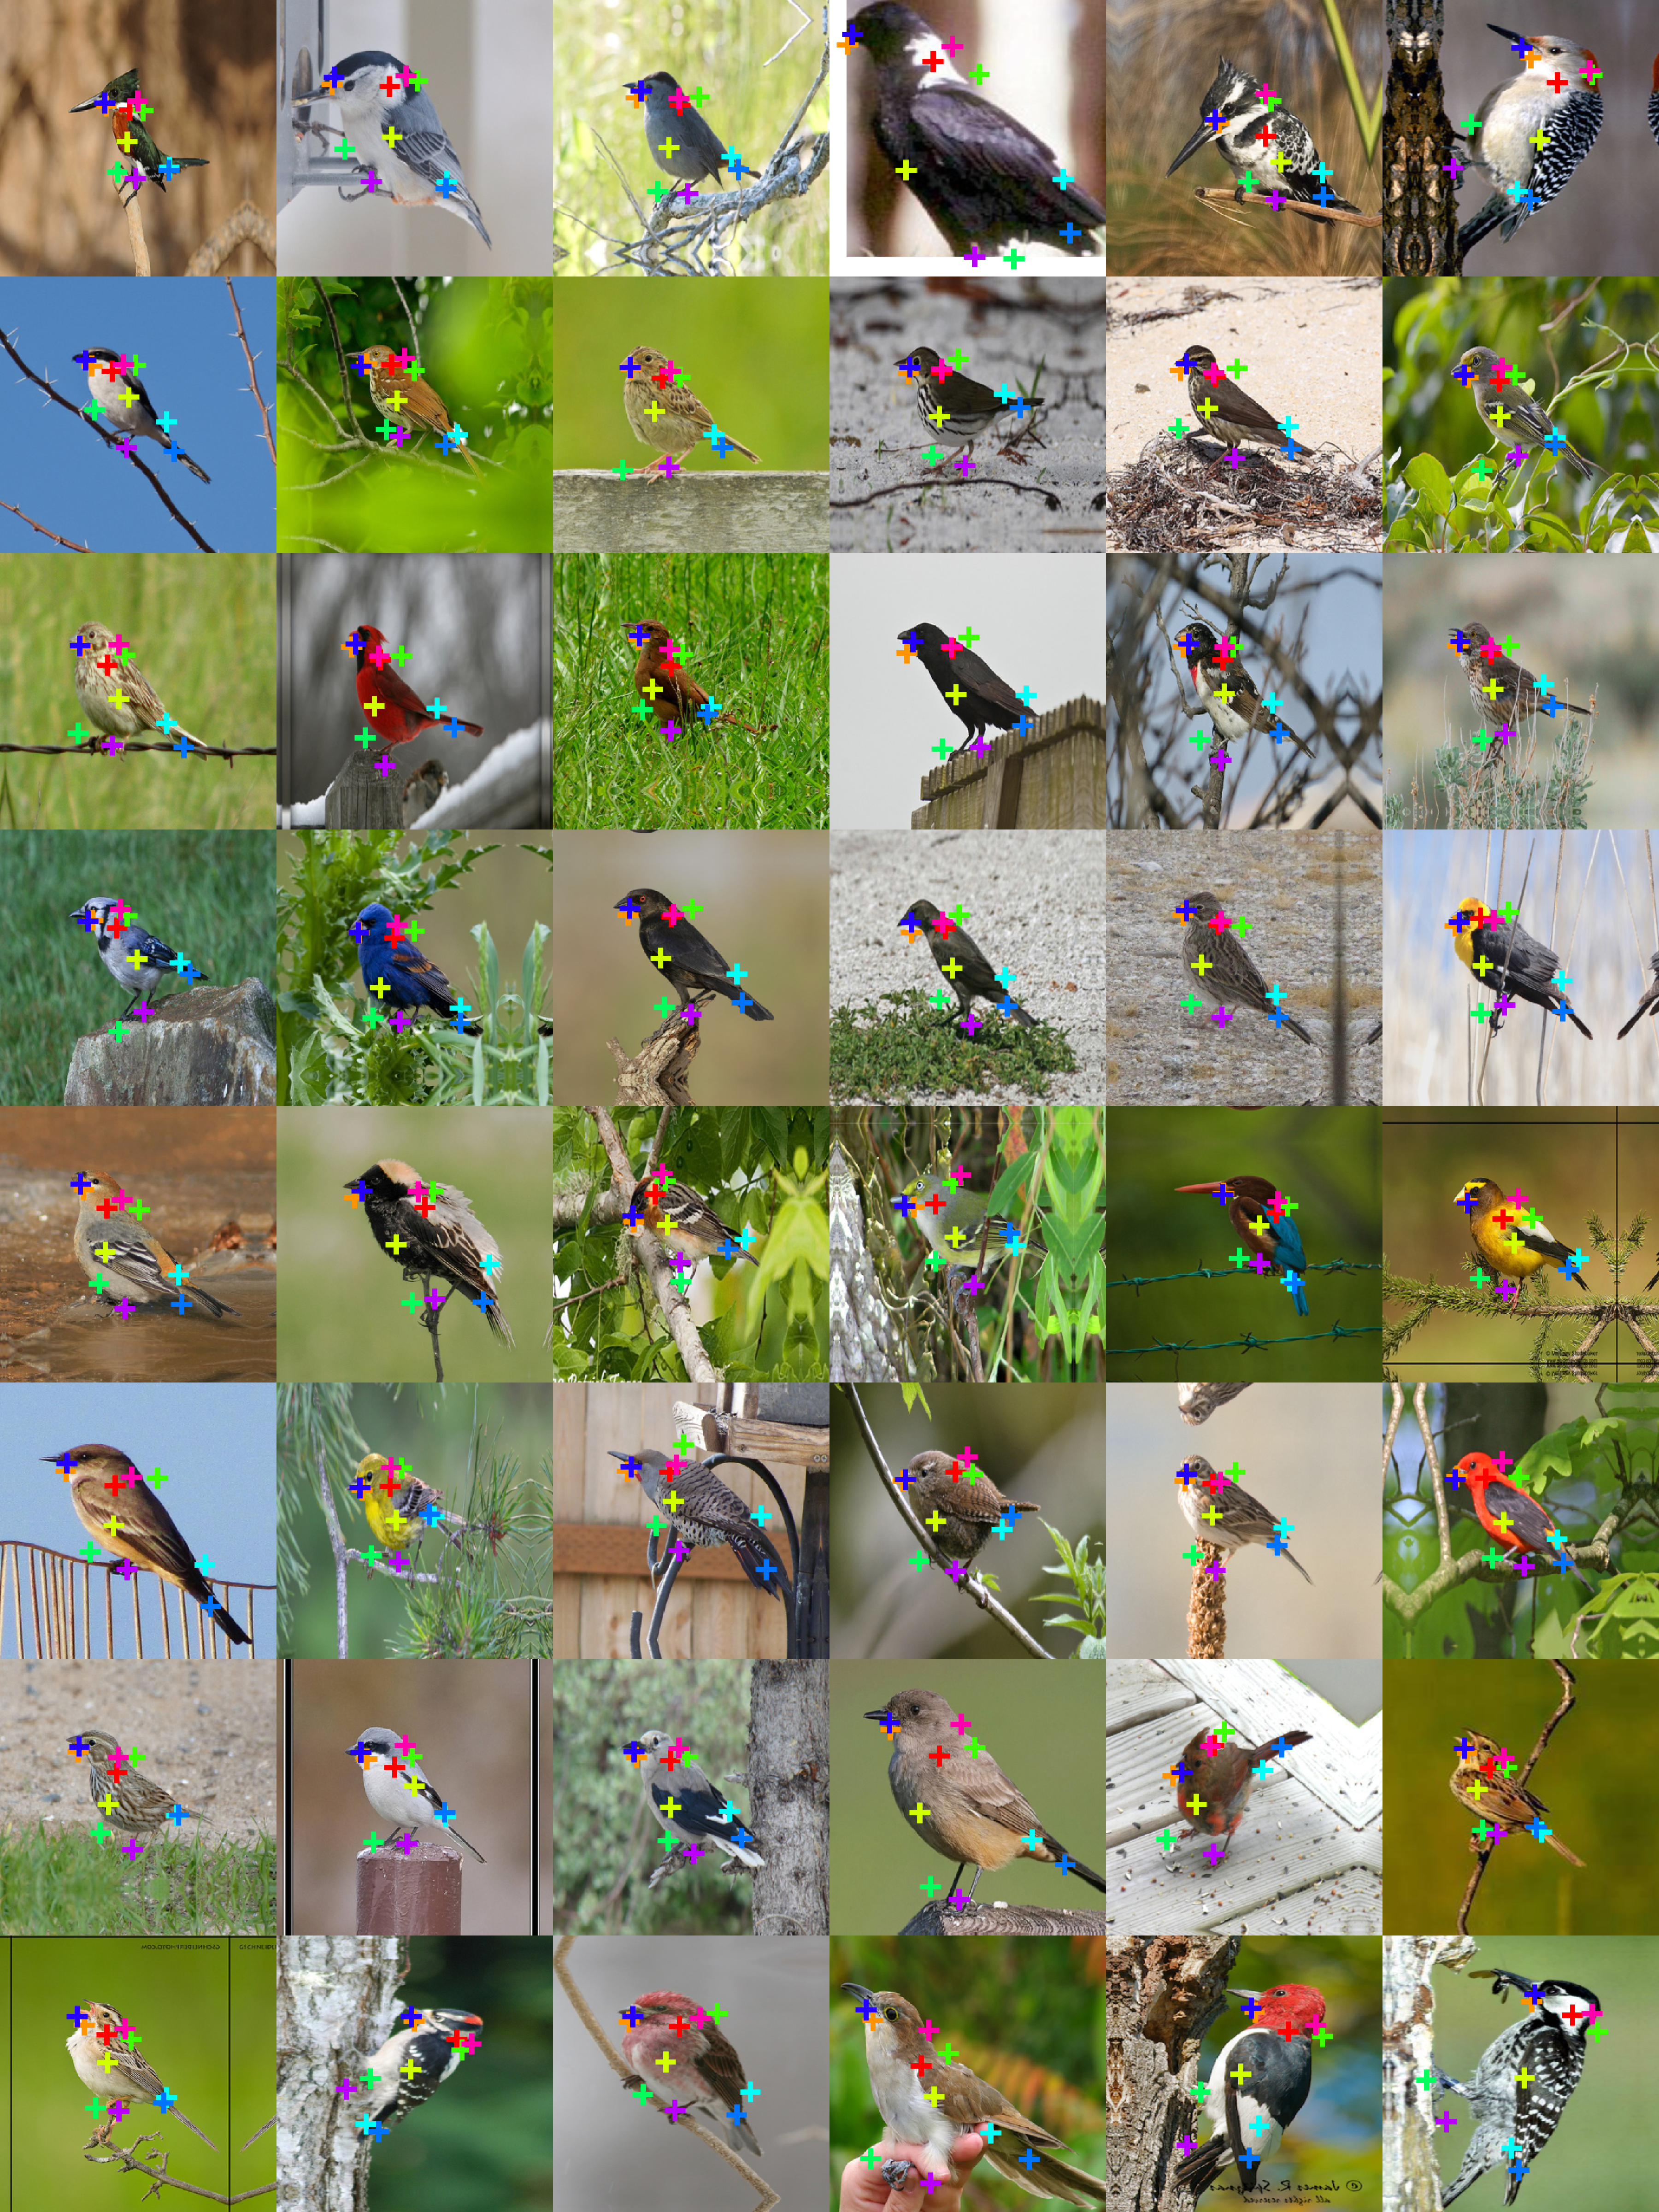
\includegraphics[trim={0cm 0cm 0cm 0cm},clip, width=1.\linewidth]{fig/supp/select48birds}
	\caption{Discovering 10 landmarks on CUB-200-2011..}
	\label{fig:kp_birds}
\end{figure}

\begin{figure}[t]
	\centering
	\includegraphics[trim={0cm 0cm 0cm 0cm},clip, width=1.\linewidth]{fig/supp/select48celeba}
	\caption{Discovering 10 landmarks on CelebA.}\label{fig:kp_celeba}%
	\label{fig:kp_celeba}
\end{figure}

\begin{figure}[t]
	\centering
	\includegraphics[trim={0cm 0cm 0cm 0cm},clip, width=1.\linewidth]{fig/supp/select48human}
	\caption{Discovering 10 landmarks on Human3.6M.}
	\label{fig:kp_human}
\end{figure}

\begin{figure}[t]
	\centering
	\includegraphics[trim={0cm 0cm 0cm 0cm},clip, width=1.\linewidth]{fig/supp/select48penn}
	\caption{Showing 12 out of 16 landmarks on Penn Action.}
	\label{fig:kp_penn}
\end{figure}



	% \chapter{Disentangled Representation}
	% % \section{Disentangled Representation}
\paragraph{Local Appearance Transfer.}
%More results for swapping parts on the Deep Fashion dataset are shown in Fig.~\ref{fig:partswaps}, as an extension to main paper, Fig. 8. The full range of possibilities for swapping part-wise appearance and body pose is best viewed in the attached video (parttransfer.mp4).
In Fig.~\ref{fig:partswaps}, we show  results for successively swapping part appearance on the Deep Fashion dataset.
% The full range of possibilities for swapping part-wise appearance and shape is best viewed in the attached video (localtransfer.mp4).

\paragraph{Video-to-Video Translation.}
In Fig.~\ref{fig:bbc1} we show sequences of a frame-to-frame appearance-shape transfer on the BBC Pose dataset. Note that the out-of-plane rotations and fine-grained details of hands and facial expressions are accurately captured. Notice the quality (smoothness, consistency) of the transfer.
% becomes most prominent in the provided video (vid2vid.mp4).
%
\begin{figure}[b!]
    \vspace*{-1.em}
	\centering
	\begin{subfigure}{.43\linewidth}
	\includegraphics[trim={0cm 0cm 0cm 0cm},clip, width=1.\linewidth]{fig/supp/DeepF/1}
	\label{fig:part3_21}
	\end{subfigure}\hspace{0.03\textwidth}
	\vspace*{-1.em}
	\centering
	\begin{subfigure}{.43\linewidth}
	\includegraphics[trim={0cm 0cm 0cm 0cm},clip, width=1.\linewidth]{fig/supp/DeepF/6}
	\label{fig:part3_30}
	\end{subfigure}
	\vspace*{-1.em}
	\centering
	\begin{subfigure}{.43\linewidth}
	\centering
	\includegraphics[trim={0cm 0cm 0cm 0cm},clip, width=1.\linewidth]{fig/supp/DeepF/2}
	\label{fig:part3_30}
	\end{subfigure}\hspace{0.03\textwidth}
	\label{fig:partswaps2}
	\centering
	\begin{subfigure}{.43\linewidth}
	\centering
	\includegraphics[trim={0cm 0cm 0cm 0cm},clip, width=1.\linewidth]{fig/supp/DeepF/4}
	\label{fig:part3_21}
	\end{subfigure}
	\centering
	\begin{subfigure}{.43\linewidth}
	\centering
	\includegraphics[trim={0cm 0cm 0cm 0cm},clip, width=1.\linewidth]{fig/supp/DeepF/3}
	\label{fig:part3_30}
	\end{subfigure}\hspace{0.03\textwidth}
	\centering
	\begin{subfigure}{.43\linewidth}
	\centering
	\includegraphics[trim={0cm 0cm 0cm 0cm},clip, width=1.\linewidth]{fig/supp/DeepF/7}
	\label{fig:part3_30}
	\end{subfigure}
	\caption{
	Successively altering the appearance of individual parts. We show 6 examples of successively altering appearances of parts using different source images. In each example we start from the original appearance (left-most column). The top row shows ground-truth images (taken from the test-set), which act as the source for the part appearance to be altered. The bottom row then illustrates the new synthesized image, which is generated based on the already altered part appearances plus the current appearance modification. Part appearances are altered in fixed order: head, upper body, legs, feet.
	}
	\label{fig:partswaps}
\end{figure}
% \newpage

\begin{figure}[b!]
	\centering
	% \begin{subfigure}{.49\linewidth}
	\centering
	\includegraphics[trim={0cm 0cm 0cm 0cm},clip, width=.8\linewidth]{fig/supp/bbc}
	% \end{subfigure}\hspace{0.01\textwidth}
	% \centering
	% \begin{subfigure}{.49\linewidth}
	% \centering
	% \includegraphics[trim={0cm 0cm 0cm 0cm},clip, width=1.\linewidth]{fig/supp/bbc_new2}
	% \end{subfigure}
	\caption{Generated sequence on BBC Pose from a target pose sequence (leftmost column) and target appearances (top row). }
	\label{fig:bbc1}
\end{figure}



	% \chapter{Implementation Details}
	% % \section{Implementation Details and Settings}

\begin{table}[h!]
	\centering
	\begin{tabular}{l|cccc}
		\hline
		Dataset & $\#$ landmarks&  res. & lr.  &  advers. \\ \hline
		Cat Head \cite{zhang08cathead} & 10\ /\ 20 & $128\times128$ &  0.001   &  \ding{55}\\
		% Cat Head & 20&  1.0 &5.0&0.001    \\
		CelebA \cite{liu15facewild}  & 10  & $128\times128$  &0.001  &  \ding{55}\\
		% CelebA & 30 &  1.0 &5.0&0.001   \\
		Human3.6M \cite{ionescu14human36m}& 16  & $128\times128$  &  0.0002  &  \ding{55}  \\
		Penn Action \cite{zhang13penn} & 16 &  $128\times128$  & 0.0002  &   \ding{55}\\
		Dogs Run (own) & 12 &   $128\times128$  & 0.001 &  \ding{55} \\
		CUB-200-2011 \cite{wah11birds}& 10 &   $128\times128$ & 0.001   &   \ding{55}\\
		BBC Pose Regression \cite{charles13bbcpose} & 30&  $128\times128$ &0.001   &  \ding{55} \\
		BBC Pose Synthesis \cite{charles13bbcpose} & 40&  $256\times256$ & 0.001   &  \ding{51}\\
		Deep Fashion  \cite{liu16deepfashion, liu16deepfashionwild} & 16 &  $256\times256$ & 0.001  &  \ding{51}  \\

	\end{tabular}
	\caption{Settings for different experiments: number of landmarks, input resolution, learning rate of Adam optimizer, adversarial task }
	\label{tab:hypers}
\end{table}


\paragraph{Implementation Details.}
	Table \ref{tab:hypers} gives an overview over the different settings for the datasets we used in our experiments.

	The architecture of the encoder for shape $E_{\sigma}$ and appearance $E_{\alpha}$ is based on the implementation %\cite{Walidtf}
	of the stacked hourglass architecture \cite{newell16hourglass}.
	In a first step the image with input resolution $h \times w \times 3$ is processed by a series of convolutions to image features of dimension $64 \times 64 \times 256$.
	The hourglass modules of $E_{\sigma}$ and $E_{\alpha}$ operate on a maximal resolution of $64 \times 64$, thus part activation maps and the localized image appearance encoding both have a spatial dimension of $64 \times 64$.
	$E_{\sigma}$ reaches its lowest resolution at $4 \times 4$ pixels whereas $E_{\alpha}$ has its lowest resolution at $32 \times 32$ pixels.
	All residual blocks of the hourglass modules have $256$ feature channels.
	The decoder is a variant of a U-Net \cite{ronneberger15unet} operating at a resolution of $h \times w$ pixels.
	Different from a standard U-Net we do not learn the downsampling stream.
	Through skip connections the approximate part activations maps are passed to the up-sampling stream with the appropriate resolutions.
	We distribute the local appearance encoding together with the corresponding approximate part activation maps into a multi-scale bottleneck of resolution $4 \times 4$ to $16 \times 16$ in the U-Net.
	The convolutional filters in the first up-sampling stage of the U-Net have $512$ feature channels.
	The number of feature channels is halved every two up-sampling stages.
	\\
	%\textbf{Local Loss.}
\paragraph{Local Loss.}
	The $\ell_1$ reconstruction loss \todo{insert reference}is weighted locally around the part activations $\sigma^i(\mathbf{x})$. For this, we multiply the loss with a soft mask. %, which is nonzero in the neighborhood of each part shape.
	For an image $\mathbf{x}$ at pixel $u$ the mask takes the form:
	\begin{equation}
		\textrm{mask}[u] = \text{min}\big(\sum_i  \frac{1}{1 + \lVert u -  \mu[\sigma^i(\mathbf{x})]/\lambda_\text{scal} \rVert}, 1\big),
	\end{equation}
	where $\lambda_\text{scal}$ is a hyperparameter.
	We do not propagate gradients through the means $\mu([\sigma^i(\mathbf{x})])$ of the mask.\\
	%\textbf{Decoder Approximation.}


	%=(
	%As denoted in (Sect. 3), the decoder receives approximated part activation maps %shapes %
	%$\tilde{\sigma}_i(a(x))$ (Eq. 7).
	%\begin{equation}
	%\tilde{\sigma}_i(a(x))[u] = \frac{1}{1 + (u -\mu_i)^T \Sigma_i^{-1} (u - \mu_i)},
	%\end{equation}
	%where $\mu_i$ and  $\Sigma_i$ denote the mean and covariance of the normalized part activation maps $\sigma_i(a(x))/\sum_{u \in \Lambda} \sigma_i(a(x))[u]$.
	%We utilize two variants for this approximation: \emph{i)} $\Sigma_i$ is set fixed to the identity matrix
	%\emph{ii)} $\Sigma_i$ is the covariance of $\sigma_i(a(x)$. In practice \emph{i}) leads to more confined part shapes.



\paragraph{Adversarial Task.}
	To improve the quality of image generations, we implement a variant of the adversarial task, as presented in \cite{isola17image2image}: A discriminator is trained to classify $N \times N$ image patches as real or fake.
	Using the mean locations of part shapes as center points, we extract image patches of size $49 \times 49$ from the real image $\mathbf{x}$ and the generated image $\hat{\mathbf{x}}$. As conditioning, the discriminator is additionally provided with corresponding patches extracted on the stack of approximated part activations $\tilde{\sigma}^i(\mathbf{x})$. The discriminator is implemented as a lightweight CNN architecture consisting of 4 convolution layers with stride 2 followed by a dense layer.
	The adversarial task is trained simultaneously with the main objective function\todo{insert reference}, no subsequent fine-tuning step is necessary.

	% \chapter{Dataset Preprocessing}
	% \section*{CelebA}{CelebA} \cite{liu15facewild} contains ca. 200k celebrity faces of 10k identities.
We resize all images to $128\times 128$ and exclude the training and test set of the MAFL subset, following \cite{thewlis17}.
As  \cite{thewlis17, zhang18}, we train the regression (to 5 ground truth landmarks) on the MAFL training set (19k images) and test on the MAFL test set (1k images).

\section*{Cat Head}{Cat Head} \cite{zhang08cathead}  has nearly 9k images of cat heads.
We use the train-test split of \cite{zhang18} for training (7,747 images) and testing (1,257 images).
We regress 5 of the 7 (same as \cite{zhang18}) annotated landmarks.
The images are cropped by bounding boxes constructed around the mean of the ground truth landmark coordinates and resized to $128\times128$.


\section*{CUB-200-2011}{CUB-200-2011} \cite{wah11birds} comprises ca. 12k images of birds in the wild from 200 bird species.
We excluded bird species of seabirds, roughly cropped using the provided landmarks as bounding box information and resized to $128\times128$.
We aligned the parity with the information about the visibility of the eye landmark.
For comparing with \cite{zhang18} we used their published code.


\section*{BBC Pose}{BBC Pose} \cite{charles13bbcpose} contains videos of sign-language signers with varied appearance in front of a changing background. Like \cite{jakab18} we loosely crop around the signers.
The test set includes 1000 frames and the test set signers did not appear in the train set.
For evaluation, as \cite{jakab18}, we utilized the provided evaluation script, which measures the PCK around $d=6$ pixels in the original image resolution.


\section*{Human3.6M}{Human3.6M} \cite{ionescu14human36m} features human activity videos.
We adopt the training and evaluation procedure of \cite{zhang18}.
For proper comparison to \cite{zhang18} we also removed the background using the off-the-shelf unsupervised background subtraction method provided in the dataset.


\section*{Penn Action}{Penn Action} \cite{zhang13penn} contains 2326 video sequences of 15 different sports categories.
For this experiment we use 6 categories (tennis serve, tennis forehand, baseball pitch, baseball swing, jumping jacks, golf swing).
We roughly cropped the images around the person, using the provided bounding boxes, then resized to $128\times128$.


\section*{Dogs Run}{Dogs Run} is made from dog videos from YouTube totaling in 1250 images under similar conditions as in Penn Action. The dogs are running in one direction in front of varying backgrounds. The 17 different dog breeds exhibit widely varying appearances.


\section*{Deep Fashion}{Deep Fashion} \cite{liu16deepfashion, liu16deepfashionwild} consists of ca. 53k in-shop clothes images in high-resolution of $256 \times 256$. We selected the images which are showing a full body (all keypoints visible, measured with the pose estimator by \cite{cao17affinityfield}) and used the provided train-test split.
For comparison with Esser \etal \cite{esser18} we used their published code.



	% \chapter{Lists}
	% \listoffigures
	% \listoftables
	\bibliography{lib_new}{}
	% % \citestyle{egu}
	% % \bibliographystyle{ieee}
	\bibliographystyle{unsrt}
	% % \bibliographystyle{plainnat}
	% \include{frm/deposition}
	% \end{appendix}
	\end{document}
